\documentclass[10pt,letterpaper]{article}
%----------------------------------------------------------------------------------------
%	PACKAGES AND OTHER DOCUMENT CONFIGURATIONS
%----------------------------------------------------------------------------------------

\usepackage{amsmath,amsfonts,stmaryrd,amssymb} % Math packages
\usepackage{amsfonts}
\usepackage{float}
\usepackage{enumerate} % Custom item numbers for enumerations
\usepackage{mathtools}
\usepackage{mathrsfs}
\usepackage{commath}
\usepackage[ruled]{algorithm2e} % Algorithms
\newtheorem{proof}{PROOF}
\usepackage[framemethod=tikz]{mdframed} % Allows defining custom boxed/framed environments

\usepackage[T1]{fontenc}
\usepackage{bigfoot} % to allow verbatim in footnote
\usepackage{python}
\usepackage{graphicx}
\usepackage{geometry}
% \userpackage{pdfpages}

\usepackage{lipsum}


\newcommand{\overbar}[1]{\mkern 1.5mu\overline{\mkern-1.5mu#1\mkern-1.5mu}\mkern 1.5mu}
\geometry{letterpaper, portrait, margin=1.5cm}

\title{ECE421 Introduction to Machine Learning \\
    Assignment \#1 \\
    Linear and Logistic Regression}
\date{Jan 2019}
\author{
  Yan, Xuanming\\
  \texttt{xuanming.yan@mail.utoronto.ca} \\
  1001175382 \\
  Contribution: 50\%
  \and
  Wang, Chu Qing\\
  \texttt{eliza.wang@mail.utoronto.com} \\
  1001303573\\
  Contribution: 50\%
} % Author name and email address
\usepackage[utf8]{inputenc}
 
\usepackage{listings}
\usepackage{color}
 
\definecolor{codegreen}{rgb}{0,0.6,0}
\definecolor{codegray}{rgb}{0.5,0.5,0.5}
\definecolor{codepurple}{rgb}{0.58,0,0.82}
\definecolor{backcolour}{rgb}{0.95,0.95,0.92}
 
\lstdefinestyle{mystyle}{
    backgroundcolor=\color{backcolour},   
    commentstyle=\color{codegreen},
    keywordstyle=\color{magenta},
    numberstyle=\tiny\color{codegray},
    stringstyle=\color{codepurple},
    basicstyle=\footnotesize,
    breakatwhitespace=false,         
    breaklines=true,                 
    captionpos=b,                    
    keepspaces=true,                 
    numbers=left,                    
    numbersep=5pt,                  
    showspaces=false,                
    showstringspaces=false,
    showtabs=false,                  
    tabsize=2
}
 
\lstset{style=mystyle}



\begin{document}
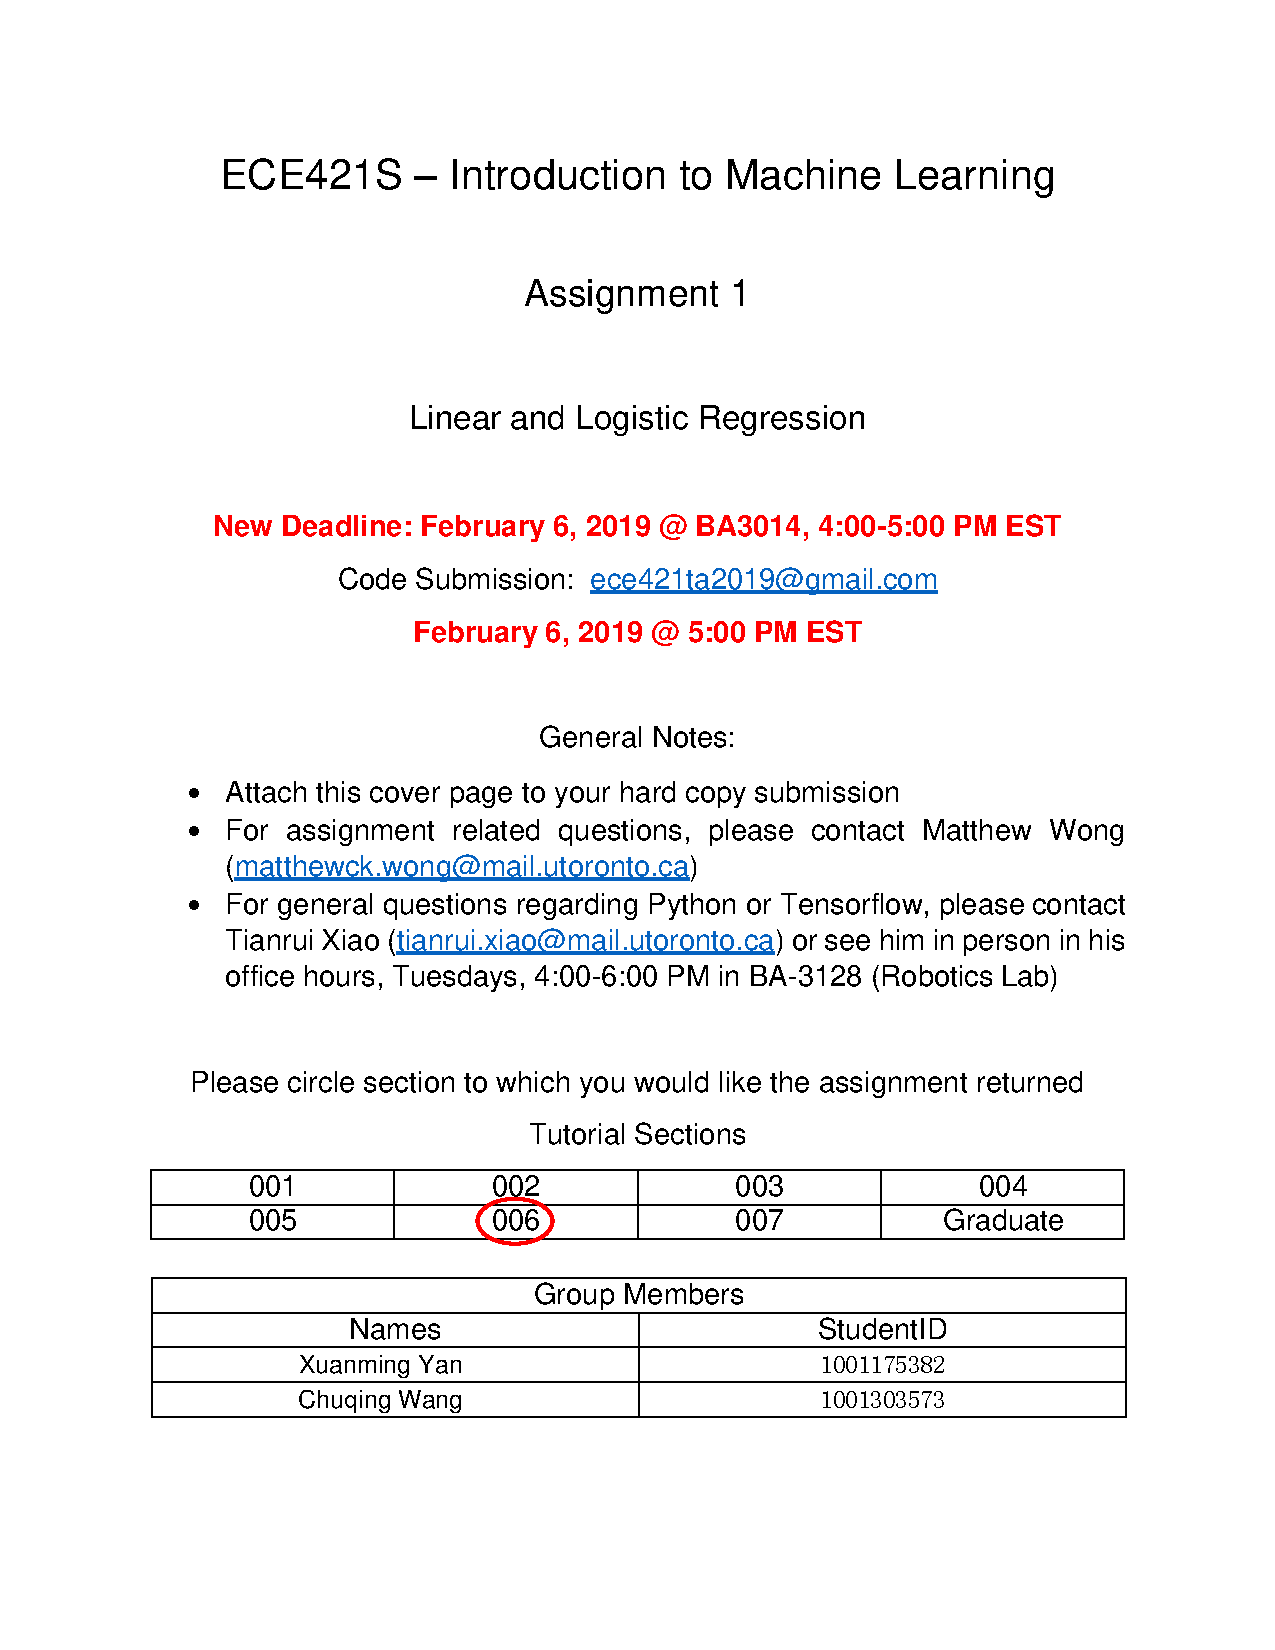
\includegraphics[width=0.95\linewidth]{a1cover.pdf}
% \includepdf[pages=-]{a1cover_updated.pdf}

\maketitle % Print the title


\section{Linear Regression}
\qquad Mean Squared Error (MSE) loss function $\mathcal{L}_{\mathcal{D}}$ and weight decay loss $\mathcal{L}_{W}$ for training a linear regression model, 
\begin{align*}
    \mathcal{L} &= \mathcal{L}_{\mathcal{D}} + \mathcal{L}_{\textbf{W}} \\
    &= \sum_{n=1}^{N}\frac{1}{2N}\left\| \textbf{W}^{T}x^{(n)} + b - y^{(n)} \right\|^{2}_{2} + \frac{\lambda}{2} \left\| \textbf{W} \right\|^{2}_{2}
\end{align*}

\subsection{Loss Function and Gradient}

\qquad  MSE written in Python is trivial, 
\lstinputlisting[language=python, caption = MSE]{MSE.py}
\qquad From above MSE loss function $\mathcal{L}_{\mathcal{D}}$ and weight decay loss $\mathcal{L}_{W}$, we can express as: 
\begin{equation*}
    \mathcal{L}(\textbf{W}) = \frac{1}{2N}\sum_{n=1}^{N} E_{n}(\textbf{W})^{2} + \lambda \sum_{i=1}^{N} w_{i}^{2}
\end{equation*}
\qquad Where $E_{n}(\textbf{W}) = \textbf{(}\sum_{i=1}^{N}w_{i}x_{i}^{(n)}\textbf{)} + b - y^{(n)}$. The goal is to choose $w_{1}$, $w_{2}$, $\dots$, $w_{D}$ and $b$ to minimize $\mathcal{L}$. In order to solve the optimization problem, we'll need to use partial derivatives. Take derivatives of $\mathcal{L}$ with respect to each element's weight, we have: 
\begin{align*}
    \frac{\partial \mathcal{L}}{\partial w_{i}} &= \frac{1}{N} \textbf{(}\sum_{n=1}^{N} E_{n}(a)  x_{i}^{(n)}\textbf{)} + 2\lambda w_{i} \\
    & = \frac{1}{N} \sum_{n=1}^{N} x_{i}^{(n)} \textbf{(} \sum_{i^{'}}w_{i^{'}}x_{i^{'}}^{(n)} + b - y^{(n)}\textbf{)} + 2\lambda w_{i}
\end{align*}
\qquad Take gradient of $\mathcal{L}$ with respect to bias, we have: 
\begin{align*}
    \frac{\partial \mathcal{L}}{\partial b} &= \frac{1}{N} \textbf{(}\sum_{n=1}^{N} E_{n}(a)  x_{i}^{(n)}\textbf{)}  \\
    & = \frac{1}{N} \sum_{n=1}^{N} \textbf{(} \sum_{i^{'}}w_{i^{'}}x_{i^{'}}^{(n)} + b - y^{(n)}\textbf{)}
\end{align*}
\qquad Implement above equation in matrix from: 
\lstinputlisting[language=python, caption = gradMSE]{gradMSE.py}


\subsection{Gradient Descent Implementation}

\qquad Gradient Descent is one of the most trivial way for optimization. It minimizes cost function in an iterative approach. To do gradient descent, we initialize the weight and bias using Gaussian distribution with mean 0 and variance 1, and repeatedly adjust them in the direction of most decreases the cost function. We repeat this procedure until the iterates converge, or stop changing much. \\

Gradient is just the direction of steepest ascent of a function. The entries of the gradient vector are simply the partial derivatives with respect to each of the variables: 
\begin{equation*}
    \frac{\partial \mathcal{L}}{\partial \textbf{W}}  = \begin{bmatrix} \frac{\partial \mathcal{L}}{\partial w_{i}} \\
    \vdots \\
    \frac{\partial \mathcal{L}}{\partial w_{D}} 
    \end{bmatrix}
\end{equation*}

Then we can formalize this using the update rule shown below, which is Gradient Descent: 
\begin{equation*}
    \textbf{W} \leftarrow \textbf{W} - \alpha \frac{\partial \mathcal{L}}{\partial \textbf{W}}
\end{equation*}

The constant $\alpha$ is known as a learning rate. The larger it is, the larger a step we take. 
\lstinputlisting[language=python, caption = grad descent]{grad_descent.py}

\subsection{Tuning the Learning Rate}


\qquad This table below shows final accuracy after 5000 epochs,
\begin{table}[H]
\centering
\begin{tabular}{|c|c|c|c|}
\hline
 \lambda = 0  & \alpha = 0.005      & \alpha = 0.001      & \alpha = 0.0001     \\ \hline
Training data accuracy & 0.644 & 0.5771428571428572              & 0.5225714285714286 \\ \hline
Valid data accuracy    & 0.62               & 0.58               & 0.54               \\ \hline
Test data accuracy     & 0.6137931034482759 & 0.47586206896551725 & 0.5103448275862069 \\ \hline
\end{tabular}
\caption{Training, validation and test losses with respect to different learning rate.}
\end{table}

\qquad We initialize the weight and bias using Gaussian distribution with mean 0 and and standard deviation 1, and $\lambda = 0$. Fig 1 shows the learning curves and accuracy using different learning rates among training, validation and test sets. Table 1 shows the final accuracy. According to these data, we could easily conclude that the model performs the best when $\alpha = 0.005$. It provides the highest accuracy and lowest loss on both training and validation sets and also converges faster than the other two. We also observe that $\alpha = 0.0001$ produces a low quality result comparing to the other two because it makes very slow as approaching the global minimum. \\

Thus, since all three models have looked through the same amount of training data (5000 epochs), a relatively large training rate is a good choice in order to achieve convergence faster. One thing we noticed from this model is that we cannot reach very high accuracy if we train this model only 5000 epochs. Therefore, We have also performed experiment with very large training epoch (100000 epochs) to debug the model, and found that there was no significant sign of over-fitting(but we can still notice that validation and test sets accuracy are lower to training set). This is most likely due to the fact that the model is not complex enough to fully over-fit on the full training data-set.\\





\begin{figure}[H]
\centering
  \begin{subfig}
  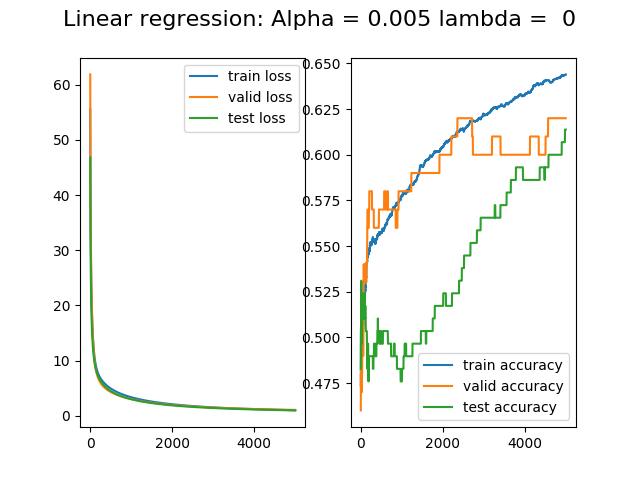
\includegraphics[width=.5\linewidth]{Linear_regression_005.png}\hfill
  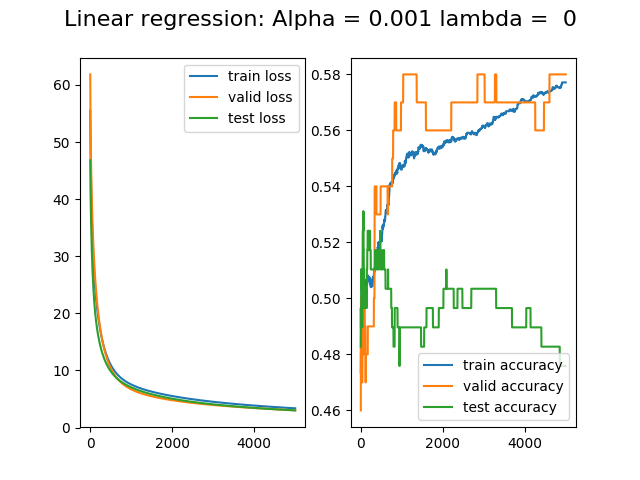
\includegraphics[width=.5\linewidth]{Linear_regression_001.png}\hfill
  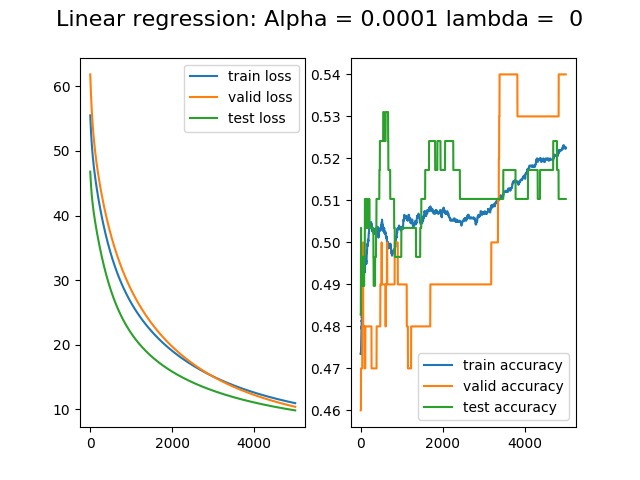
\includegraphics[width=.5\linewidth]{Linear_regression_0001.png}\hfill
  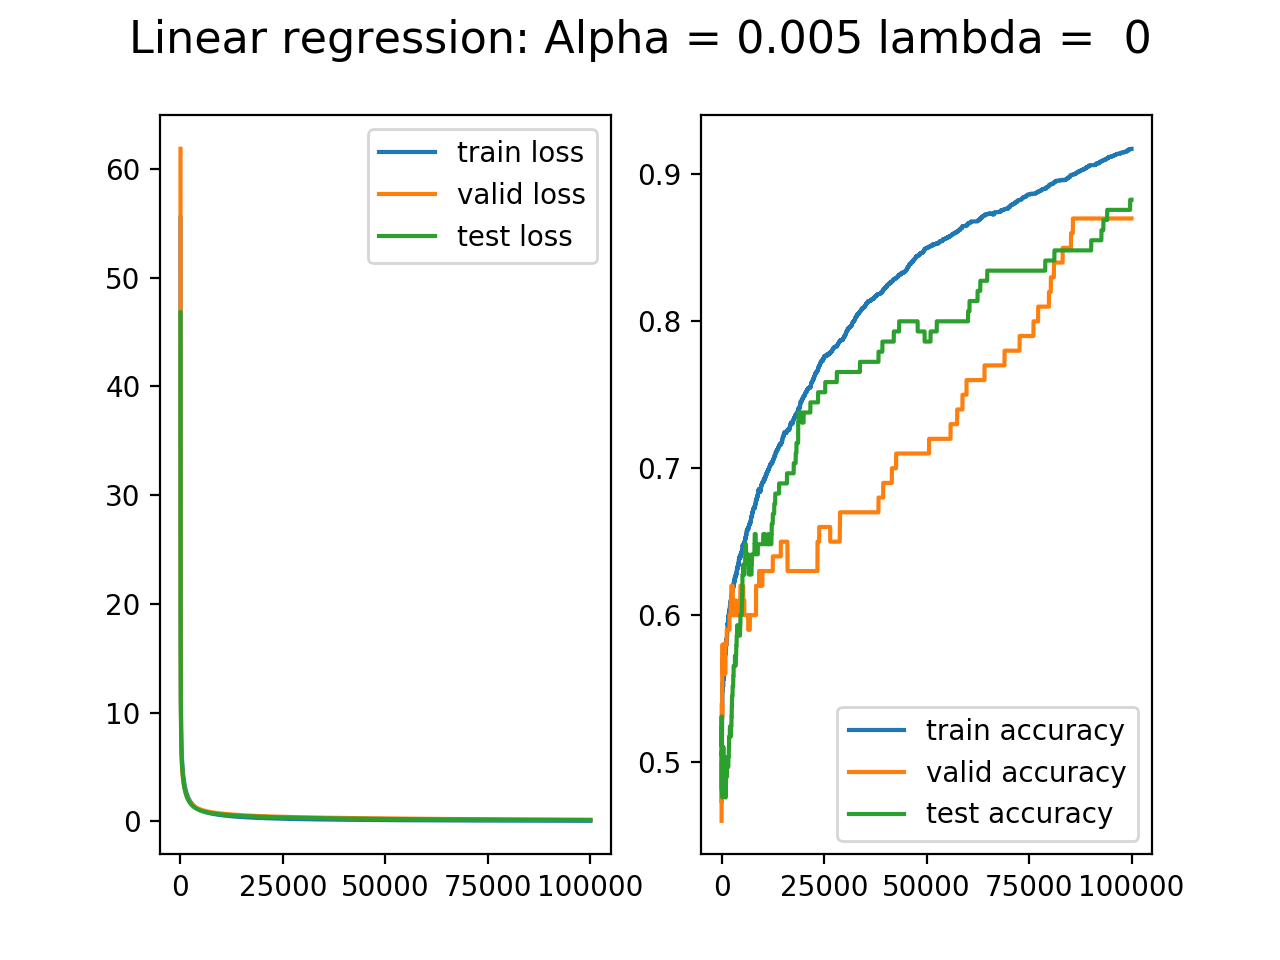
\includegraphics[width=.5\linewidth]{Linear_regression_overfitting.png}
  \caption{Training, validation and test losses with respect to different learning rate.}
  \end{subfig}
\end{figure}
 


To summarize, with smaller learning rate, classifier will take more epochs to converge. Therefore, smaller learning rate will take more time to train. However, larger learning rate can over shoot.

% \begin{figure}[h]
% \centering
%  \begin{subfig}
%   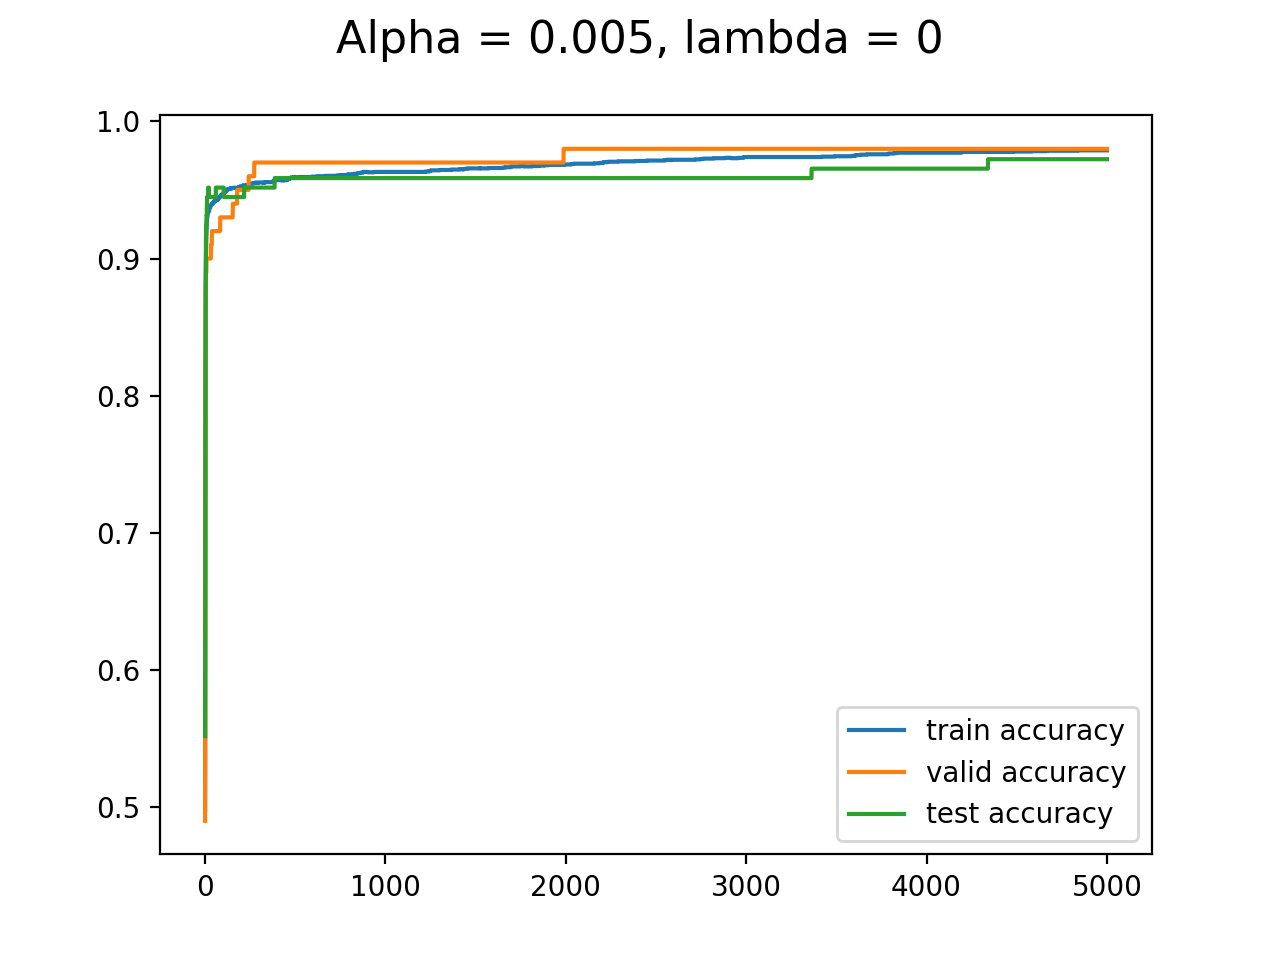
\includegraphics[width=.5\linewidth]{p1_acc.png}\hfill
%   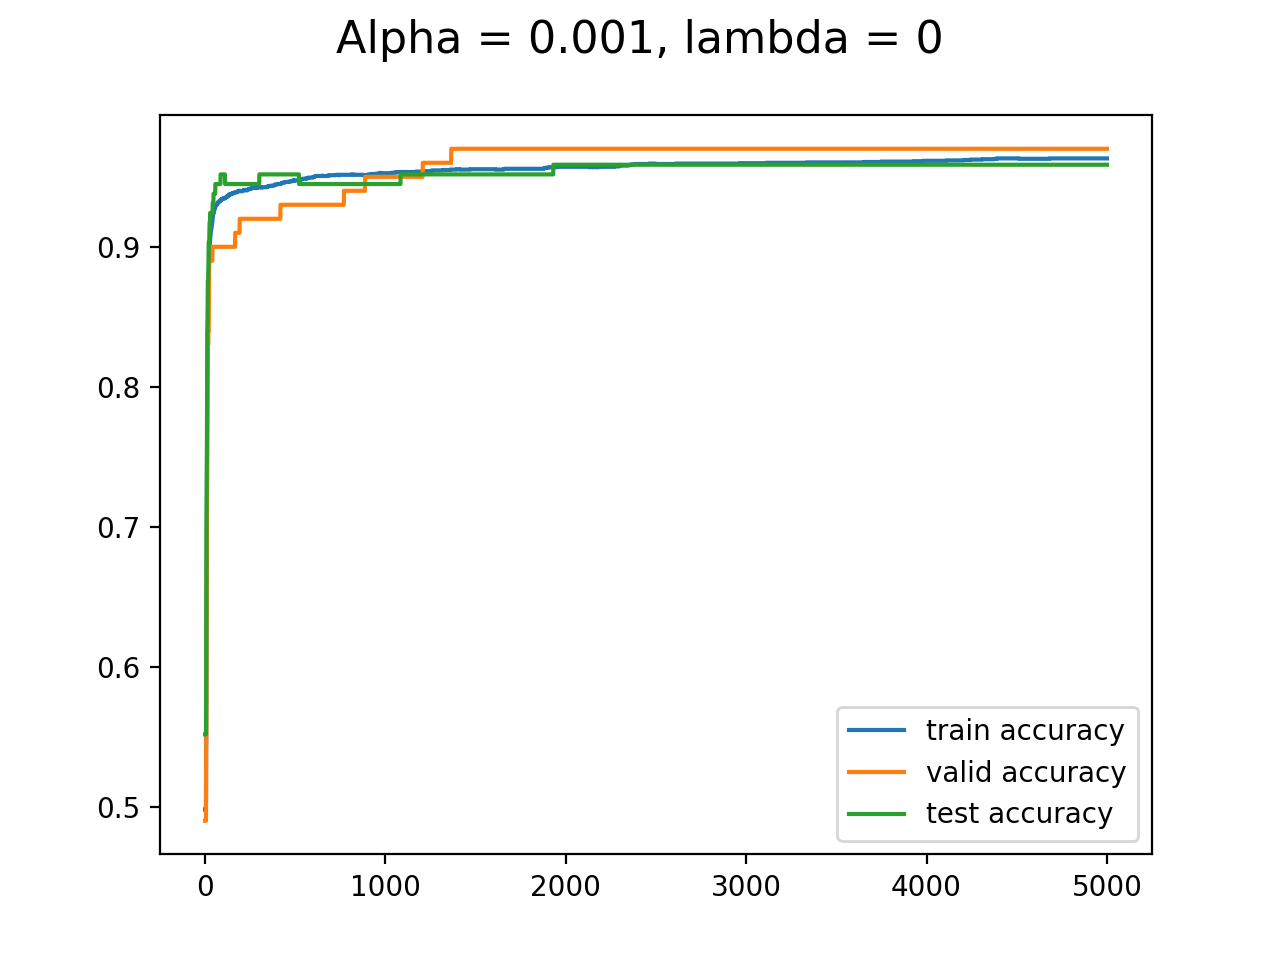
\includegraphics[width=.5\linewidth]{p2_acc.png}\hfill
%   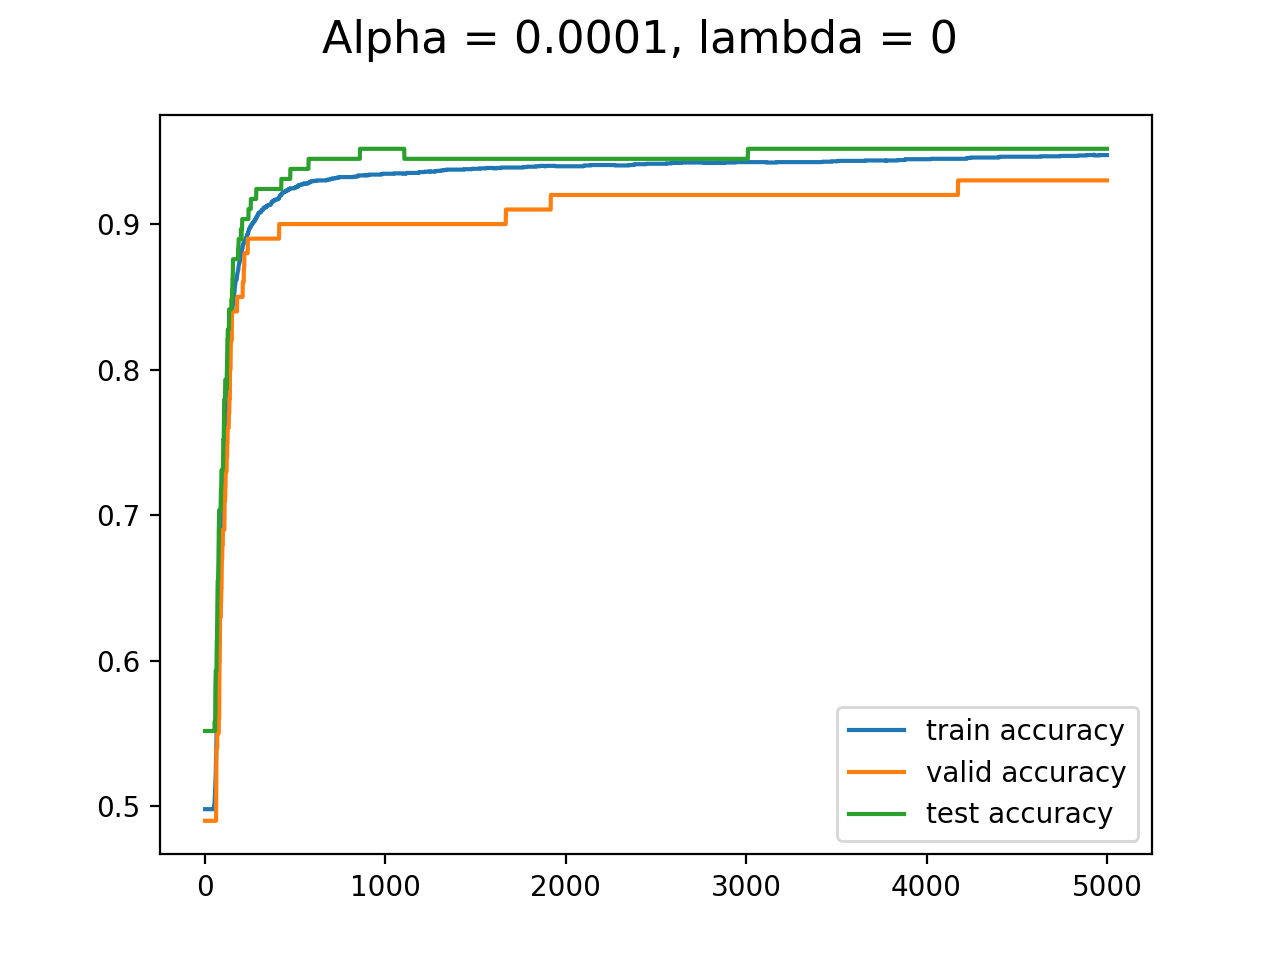
\includegraphics[width=.5\linewidth]{p3_acc.png}
%   \caption{Training, validation and test accuracy with respect to different learning rate.}
%   \end{subfig}
% \end{figure}

\subsection{Generalization}

\qquad Fig 2 shows the accuracy using different weight decays among training, validation and test sets. Table 2 shows the final accuracy on training, validation and test sets. The purpose of introducing weight decay in the model is to prevent the weight from growing too large over-fitting on the training data. \\

From previous task, we noticed that with $\alpha = 0.005$, training accuracy is higher than validating and testing accuracy. Which shows the sign of over-fitting. In order to address over-fitting, we can manually tune the weight decay value, which is $\lambda$ in this problem. We could see as $\lambda$ increases, the training loss increases, which is expected because to prevent over-fitting means to prevent extremely good fitting on training set. However, small $\lambda$ value in this model contributes little for preventing over-fitting and improve convergence speed. When $\lambda = 0.1$, we have lowest valid/test data loss and highest valid/test data accuracy, but model took about 2000 epochs to converge. Compare to $\lambda = 0.5$, which gives relatively same performance, it only took less than 500 epochs to converge. Therefore, we conclude that, $\lambda = 0.5$ provides a faster convergence and lower validation loss; therefore, we would choose $\lambda = 0.5$ as our best weight decay parameter.\\

This table below shows final accuracy after 5000 epochs,
\begin{table}[H]
\centering
\begin{tabular}{|c|c|c|c|}
\hline
  \alpha = 0.005  & \lambda = 0.001  & \lambda = 0.1     & \lambda = 0.5    \\ \hline
Training data accuracy & 0.6508571428571429 & 0.9817142857142858             & 0.9771428571428571 \\ \hline
Valid data accuracy    & 0.62               & 0.99               & 0.98               \\ \hline
Test data accuracy     & 0.6275862068965518 & 0.9862068965517241 & 0.9793103448275862 \\ \hline
\end{tabular}
\caption{Training, validation and test losses with respect to different weight decays.}
\end{table}


\begin{figure}[H]
\centering
  \begin{subfig}
  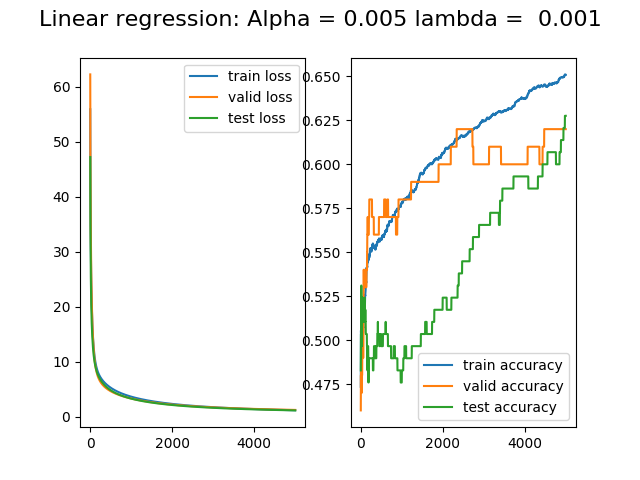
\includegraphics[width=.49\linewidth]{Reg_Linear_regression_001.png}\hfill
  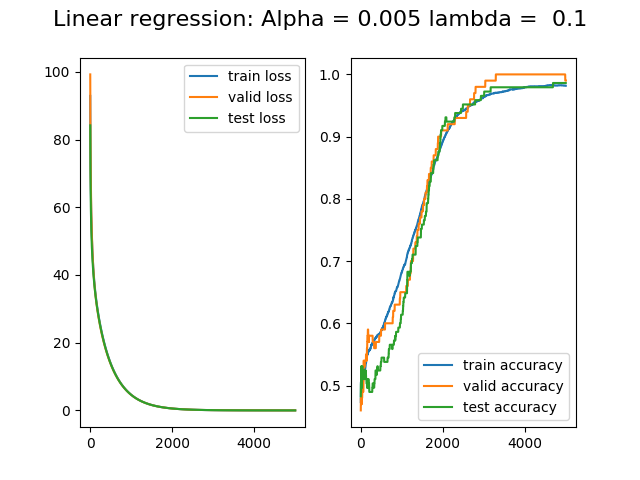
\includegraphics[width=.49\linewidth]{Reg_Linear_regression_01png.png}\hfill
  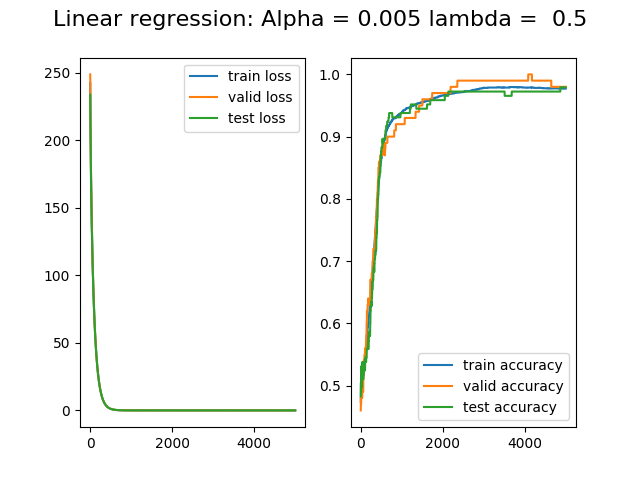
\includegraphics[width=.49\linewidth]{Reg_Linear_regression_05.png}
  \caption{Training, validation and test losses with respect to different regularization.}
  \end{subfig}
\end{figure}

\begin{figure}[H]
\centering
 \begin{subfig}
  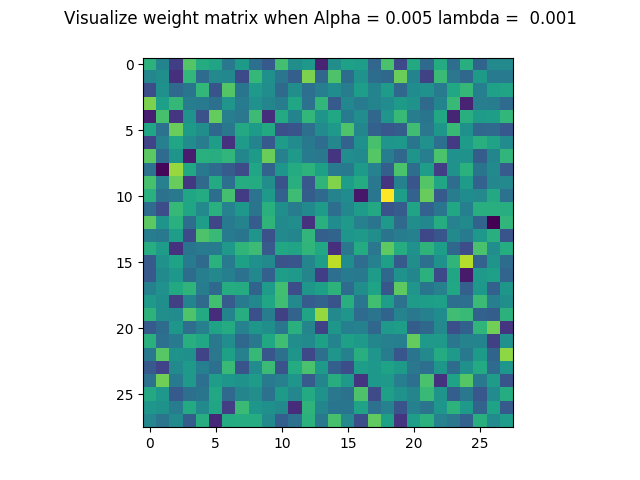
\includegraphics[width=.33\linewidth]{reg_VWM_001.png}\hfill
  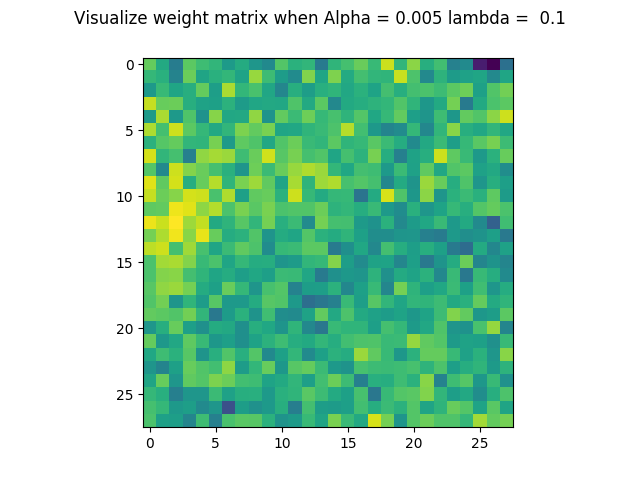
\includegraphics[width=.33\linewidth]{reg_VWM_01.png}\hfill
  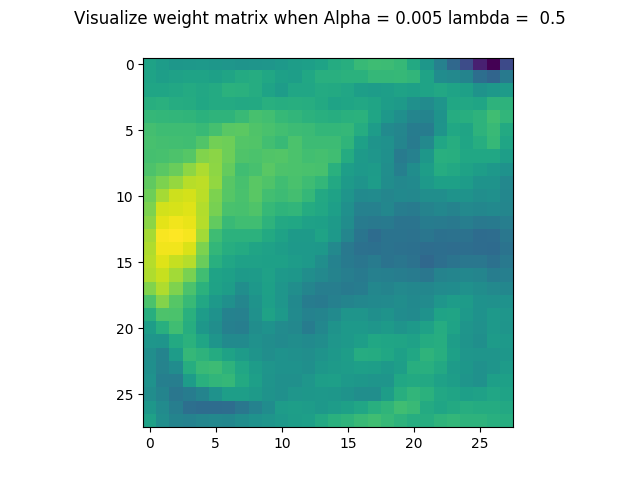
\includegraphics[width=.33\linewidth]{reg_VWM_05.png}
  \caption{Visualization of Weight matrix with different regularization.}
  \end{subfig}
\end{figure}

We can also visualize weight matrix to compare the performance of each model. Fig 3 shows visualized  weight matrix under different weight decay values. when $\lambda = 0.5$, we can easily recognize the letter "C", this shows that after model is trained, our classifier captured the most important features for this data-set. Similar to "eigenfaces" in computer vision problem of human face recognition. \\



To summaries, the meaning of regularization is to prevent the model from over-fitting on the actual data; therefore, it should sacrifice some training accuracy and improve the validation/test accuracy. The purpose of validation set is to better tune the hyper-parameters such as learning rate, weight decay, and network architecture to find the best possible model. And test set is supposed to represent the real data, which shouldn't be visible during the phase while we train and tune the model. Otherwise, the test set becomes another validation set and introduces biases while selecting the model. 

\subsection{Comparing Batch GD with normal equation}

 \qquad Table 3 below shows final training MSE, accuracy and computation time between Batch GD and normal equation. We could easily tell Normal Equation performs much better than Batch GD with zero weight decay, which is expected because the analytic solution is the optimum. Batch GD model takes about half minute to training but the Normal Equation takes less than a second to compute, Batch GD is far behind Normal Equation in this scenario.\\

But is is not always the case. 
In order to find out under what circumstances Batch GD would perform better, we need to analyze these two approaches first. If the data set contains $N$ samples and each sample has d features, the complexity of Normal Equation is $\textbf{O}(Nd^{2})$, where inverting a matrix is very expensive. It may have complexity of $\textbf{O}(d^{3})$(even though there are fancy modern numerical techniques for matrix inversion may have better complexity, it still above quadratic). And the complexity of Batch GD is $\textbf{O}(Nd \cdot iteration)$. If $N \gg d$, Batch GD would be more efficient when the data set has a large amount of data samples; otherwise,  Normal Equation would produce a better solution in a quicker way.

\begin{table}[h]
\centering
\begin{tabular}{|c|c|c|c|c|c|}
\hline
   & Running Time      &  Train data accuracy      &  Valid data accuracy &  Test data accuracy & MSE     \\ \hline
Normal equation & 0.36765 second & 99\%  & 96\% & 94\%  & 0.0094 \\ \hline
Batch GD    & 20.93 seconds  & 64.4\% & 62\%   & 61.37\%  & 1.013  \\ \hline

\end{tabular}
\caption{Comparing Batch GD with normal equation.}
\end{table}

\lstinputlisting[language=python, caption = Numpy script for optimal linear regression weights]{norm_equation.py}


\section{Logistic Regression}

The cross-entropy loss is defined as: 
\begin{align*}
    \mathcal{L} &= \mathcal{L}_{\mathcal{D}} + \mathcal{L}_{\textbf{W}} \\
    &= \sum_{n=1}^{N}\frac{1}{N}\bigg[ -y^{(n)}\log\hat{y}(\textbf{x}^{(n)}) -(1-y^{(n)})\log(1-\hat{y}(\textbf{x}^{(n)}))\bigg] + \frac{\lambda}{2} \left\| \textbf{W} \right\|^{2}_{2}
\end{align*}
Where $\hat{y}(\textbf{x}) = \sigma(W^{T}\textbf{x}+b)$. 

\subsection{Loss Function and Gradient}
 Let's consider $\mathcal{L}_{\mathcal{D}} =  -y\log\hat{y}(\textbf{x}) -(1-y)\log(1-\hat{y}(\textbf{x}))$. First, take derivatives of $\mathcal{L}_{\mathcal{D}}$ with respect to $\hat{y}(\textbf{x})$:
\setcounter{equation}{0}
\begin{equation}
    \frac{d \mathcal{L}_{\mathcal{D}}}{d \hat{y}(\textbf{x})} = -\frac{y}{\hat{y}(\textbf{x})} + \frac{1-y}{1-\hat{y}(\textbf{x})}
\end{equation}

\noindent Then, take derivative of $\hat{y}(\textbf{x})$ with respect to $\textbf{x}$:
\begin{equation}
    \frac{d\hat{y}(\textbf{x})}{d\textbf{x}} = \hat{y}(\textbf{x})(1-\hat{y}(\textbf{x}))
\end{equation}
\noindent Next, take derivative of $\textbf{x}$ with respect to weight:
\begin{equation}
    \frac{\partial \textbf{x}}{\partial W} = \textbf{x}
\end{equation}

\noindent Finally, combine equation (1), (2) and (3) and add regularization term, we have: 
\begin{equation}
    \frac{\partial \mathcal{L}_{\mathcal{D}}}{\partial W} = \frac{1}{N}\Big[\textbf{x}^{T}(\hat{y} - y) \Big] + \sum_{n=1}^{N} 2\lambda w_{i}
\end{equation}

\noindent Similarly, 
\begin{equation}
    \frac{\partial \mathcal{L}_{\mathcal{D}}}{\partial d} = \sum_{n=1}^{N}\frac{1}{N}(\hat{y} - y) 
\end{equation}
\lstinputlisting[language=python, caption = Cross Entropy Loss]{crossEntropyLoss.py}

\lstinputlisting[language=python, caption = Cross Entropy Loss Gradient]{gradCE.py}

\subsection{Learning}

\begin{figure}[H]
\centering
 \begin{subfig}
  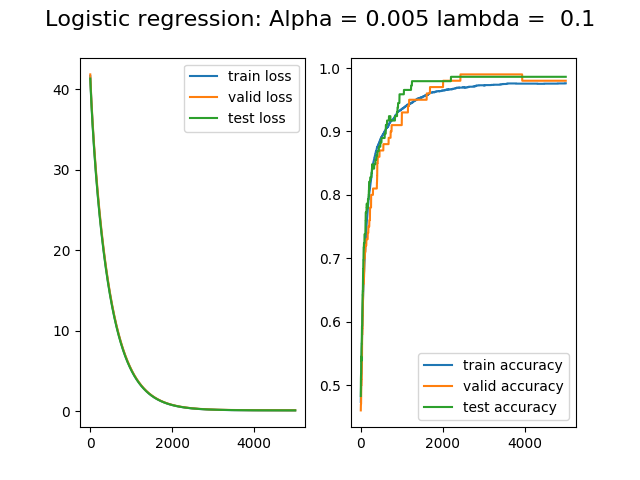
\includegraphics[width=.5\linewidth]{Reg_Logi_regression_01.png}\hfill
  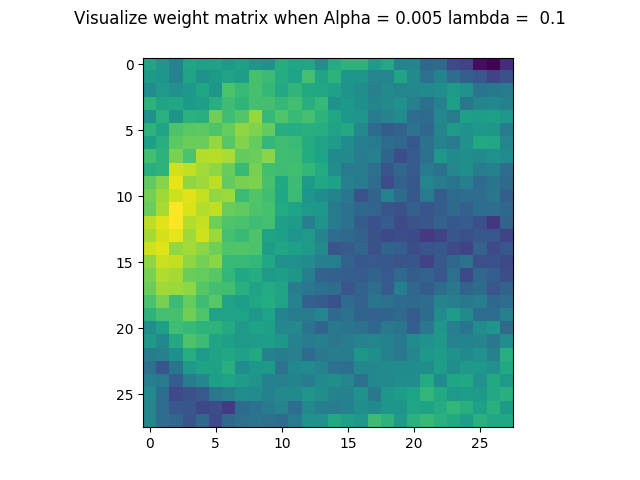
\includegraphics[width=.5\linewidth]{reg_Logi_VWM_01.png}\hfill
  \caption{Logistic regression loss and accuracy curves and Visualization of Weight matrix}
  \end{subfig}
\end{figure}

\qquad The gradient decent function that we had implemented with cross-entropy approach were similar to the gradient decent function by using MSE approach, the only difference was the replacement of MSE Loss function and gradMSE function with CrossEntropyLoss function and gradCE function. \\

The training model results were shown below in figure 4.\\

\lstinputlisting[language=python, caption = grad descent]{grad_descentCE.py}



\subsection{Comparison to Linear Regression}

\qquad Due to the reason of numerical stability, we had initialized weights by using Gaussian distribution with mean of 0, standard deviation of 0.5 for both MSE and CE. \\

Figure 5 shows the training loss for both MSE and CE approached models, for the figure, We could easily observe that logistic regression model using cross entropy loss converges much faster than linear regression model using MSE. This had indicated Cross-entropy is a batter measure than MSE for classification. This could be explained when deriving cost functions from the aspect of probability and distribution, MSE can be derived when assuming the error follows Normal Distribution, whereas the CE is based on the assumption of binomial distribution, this gives the natural that CE is better when doing classification (which is what we had done in this assignment), and MSE is better for doing regression.\\


\begin{figure}[H]
\centering
 \begin{subfig}
  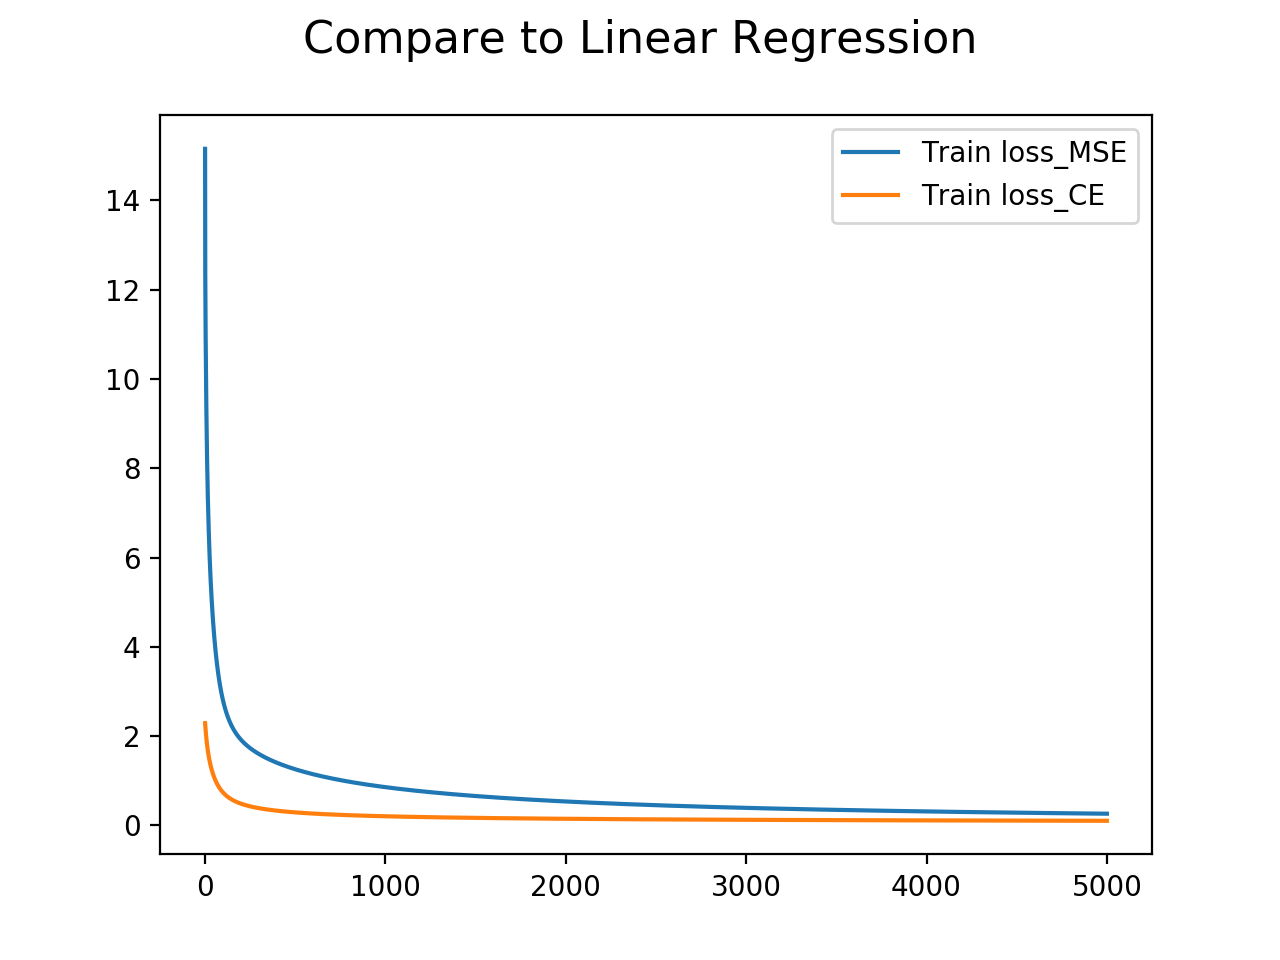
\includegraphics[width=.5\linewidth]{Comparison_loss.png}\hfill
  \caption{Training cross entropy loss and MSE loss for logistic regression and linear regression}
  \end{subfig}
\end{figure}


\section{Batch Gradient Descent vs. SGD and Adam}

\subsection{Building the Computational Graph}

\lstinputlisting[language=python, caption = Build Graph]{SGD.py}

\subsection{Implementing Stochastic Gradient Descent}

\lstinputlisting[language=python, caption = Tensorflow Session]{batch.py}

\begin{figure}[H]
\centering
 \begin{subfig}
  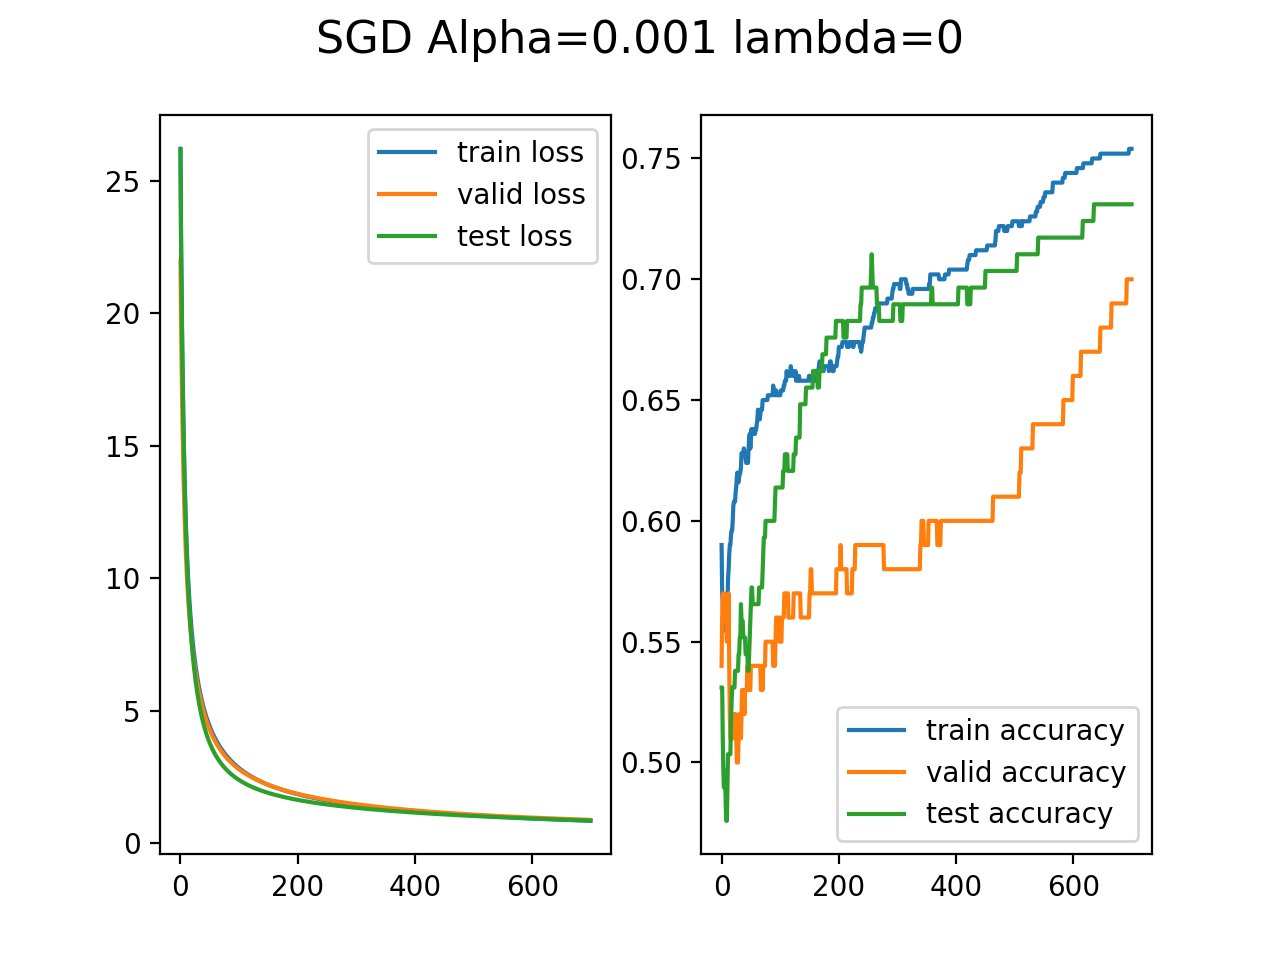
\includegraphics[width=.5\linewidth]{SGD_MSE.png}
  \caption{SGD for minibatch of 500 over 700 epochs}
  \end{subfig}
\end{figure}

\subsection{Batch Size Investigation}

\qquad Figure 7 had shown the loss and accuracy changing curves for different batch sizes (100, 700, 1350). There were not much differences between loss curves for mini batch size 100 and 700, however, as the size of the mini batch increased to 1370, the graph showed a large increase on the loss and slower decay for all three data sets. The differences between different batch size could be observed more clearly on the accuracy curves. As the batch size increased, the models generated become less on the accuracy and consistency of training, valid, and test data sets. This is because mini batch has the regularizing effects on the model in the way of adding extra noise to the gradient estimations. This helped the model to avoid bias estimations and also able to jerk the model out from local minimum, which led to better generalization. As the batch size increased, the noise become smaller, hence, there will be lose on the regularizing effect and lower the accuracy of validation and test data. \\

\begin{figure}[H]
\centering
 \begin{subfig}
  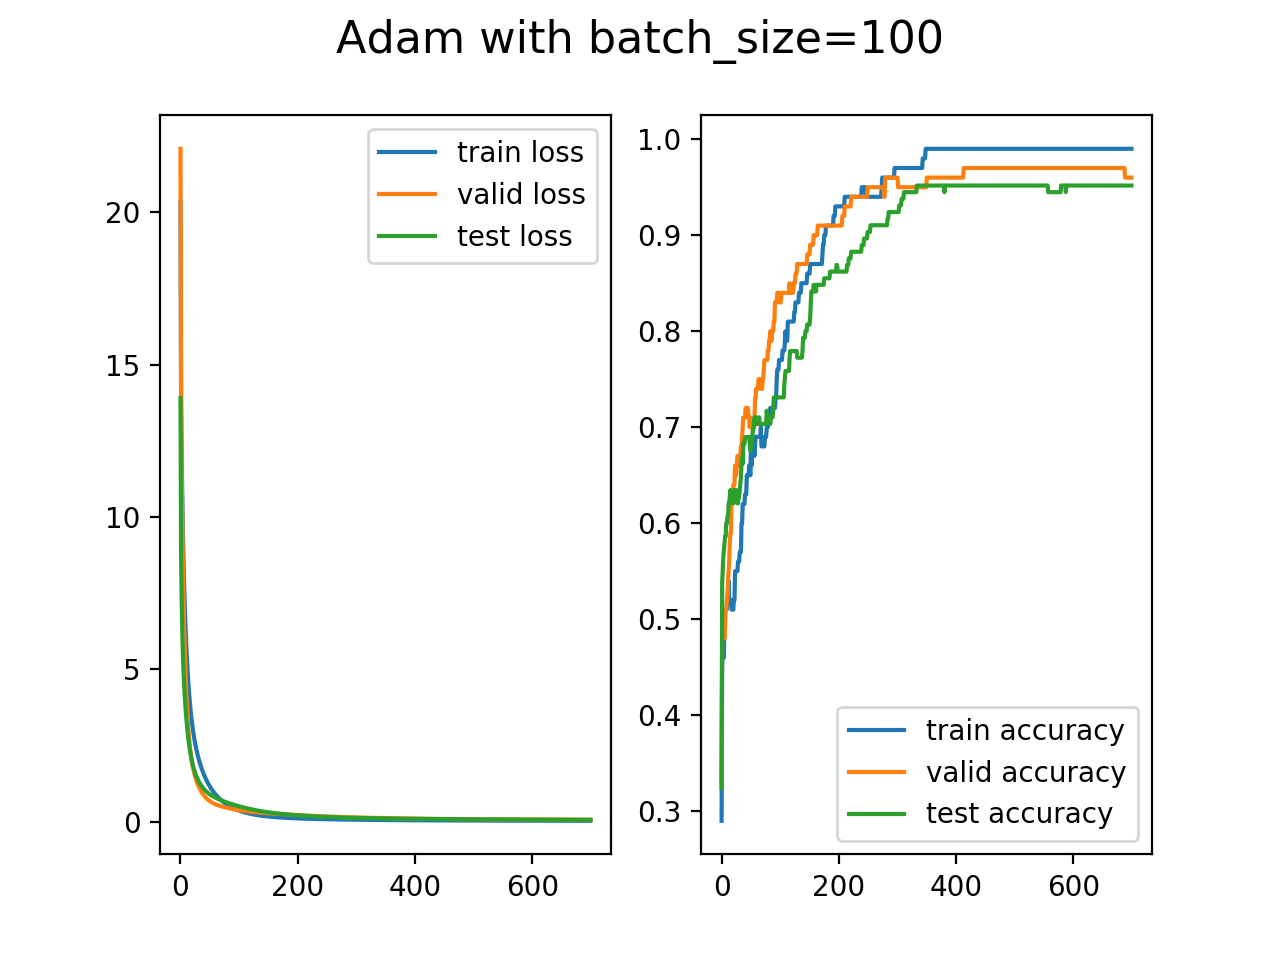
\includegraphics[width=.45\linewidth]{adam_100.png}\hfill
  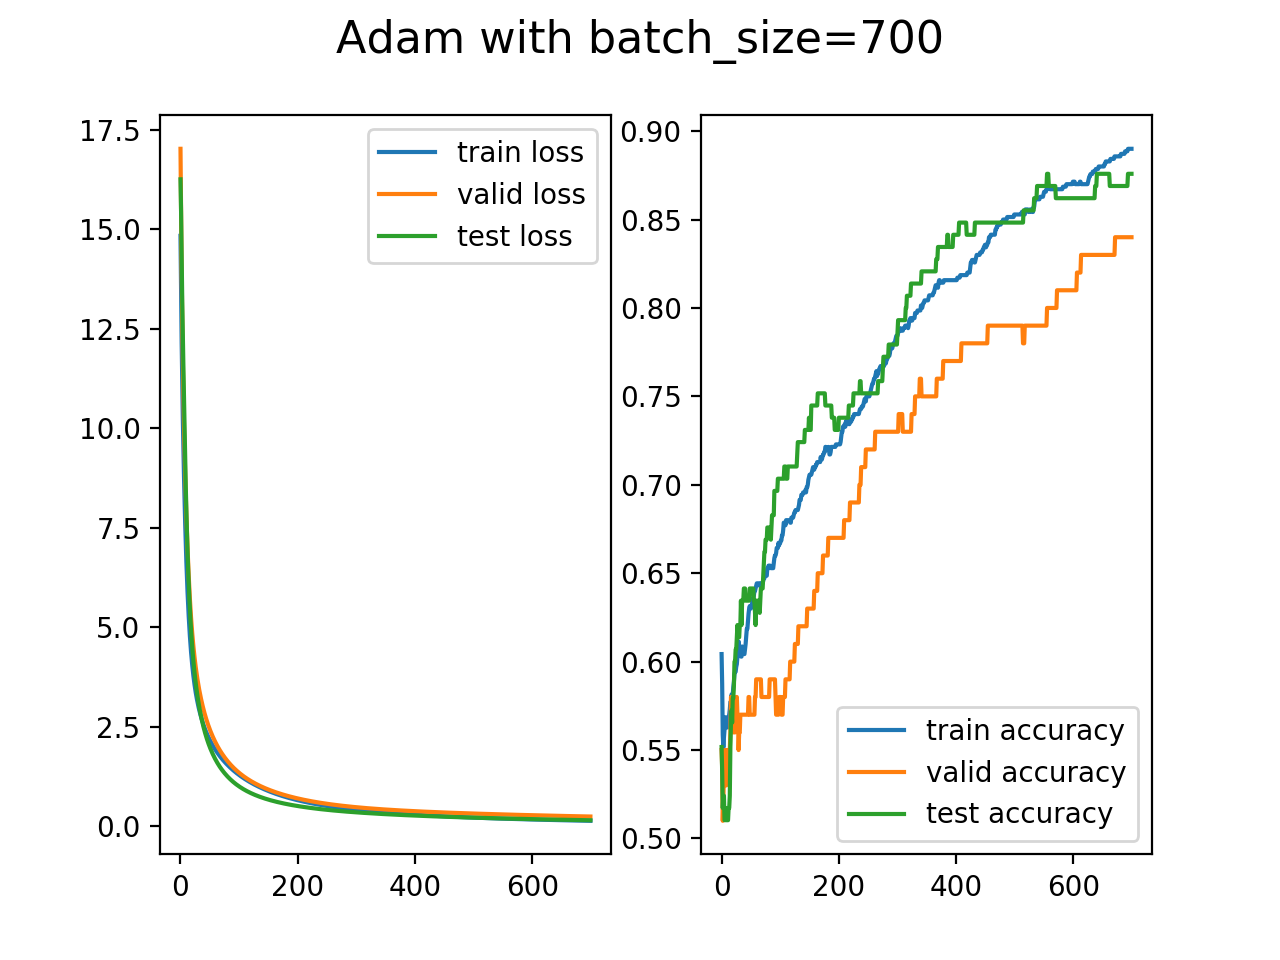
\includegraphics[width=.45\linewidth]{adam_700.png}\hfill
  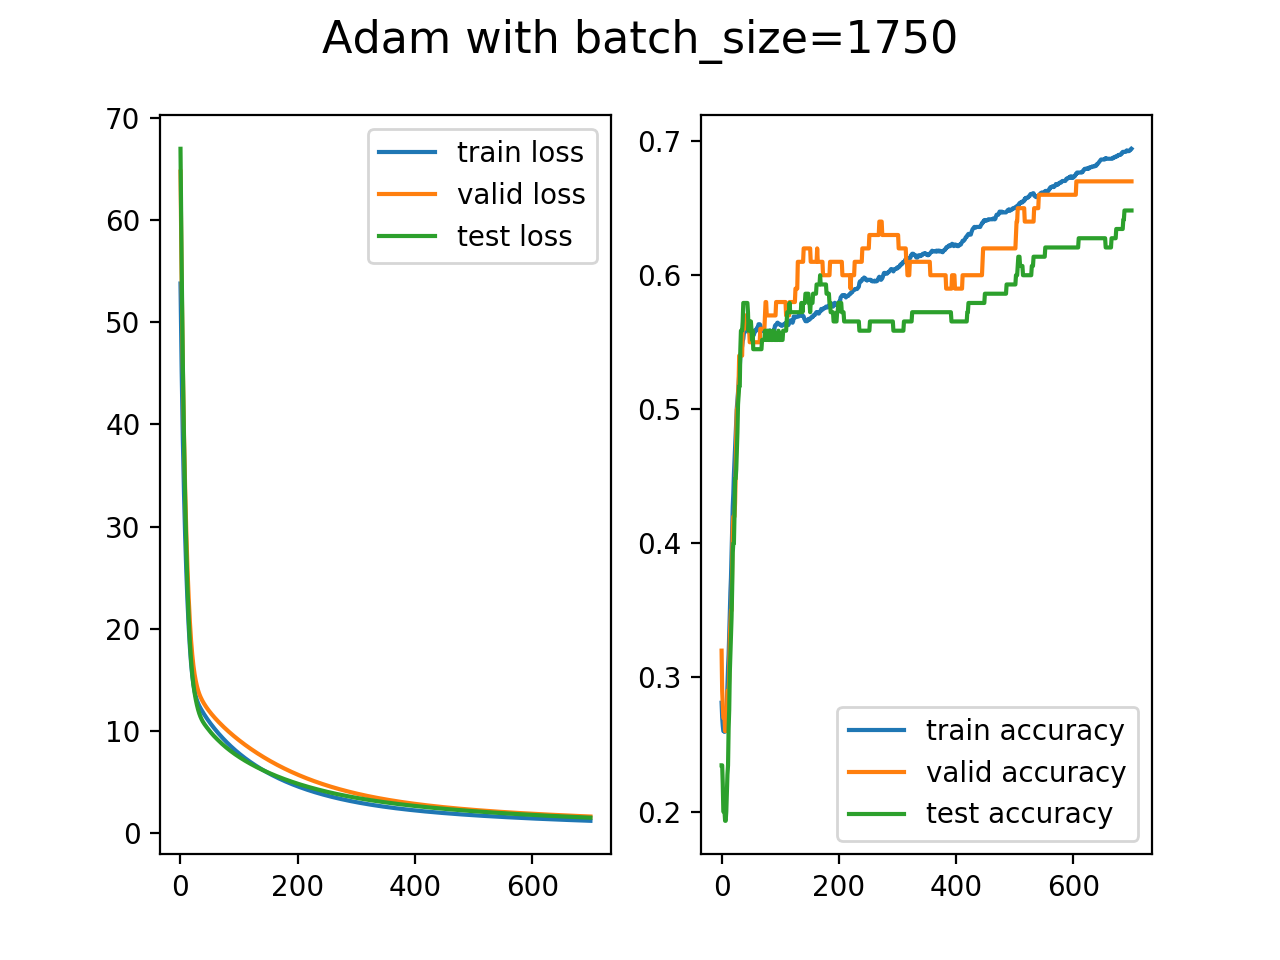
\includegraphics[width=.45\linewidth]{adam_1750.png}
  \caption{SGD optimized using Adam uising different batch size.}
  \end{subfig}
\end{figure}


\subsection{Hyperparameter Investigation}
\begin{figure}[H]
\centering
 \begin{subfig}
  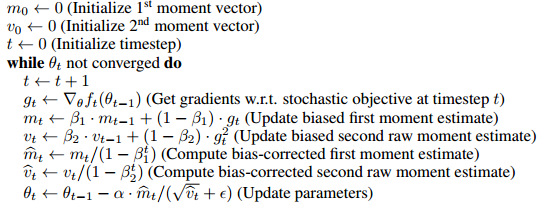
\includegraphics[width=.5\linewidth]{08VZN.png}\hfill
  \caption{Adam hyper-parameters used for optimization. \cite{2014arXiv1412.6980K}}
  \end{subfig}
\end{figure}

\qquad Figure 9 had shown the different accuracy curves' plots for train, valid, and test data in the context of changing Adam hyper-parameters $\beta_1$, $\beta_2$, and $\epsilon$ values. The default values are: \\
\begin{equation*}
    \beta_1 = 0.9 \qquad
\beta_2 = 0.999 \qquad
\epsilon = 10e-08
\end{equation*}

\begin{table}[h]
\centering
\begin{tabular}{|c|c|c|c|c|c|c|}
\hline
        &  \beta_1 = 0.95      &  \beta_1 = 0.99 &  \beta_2 = 0.99  & \beta_2 = 0.9999 & \epsilon = 1e-9 & \epsilon = 1e-4  \\ \hline
Train data accuracy & 91\% & 80\%  & 93.8\% & 77.2\%  &  89.2\% & 90.2\% \\ \hline
Valid data accuracy    & 89\% & 79\%  & 92\% & 79\%  &  83\% & 84\%   \\ \hline
Test data accuracy & 87.5\% & 82\%  & 92.4\% & 81.4\%  &  86.9\% & 84.1\% \\
\hline
\end{tabular}
\caption{Different Hyper-parameters final accuracy.}
\end{table}


\begin{figure}[H]
\centering
 \begin{subfig}
  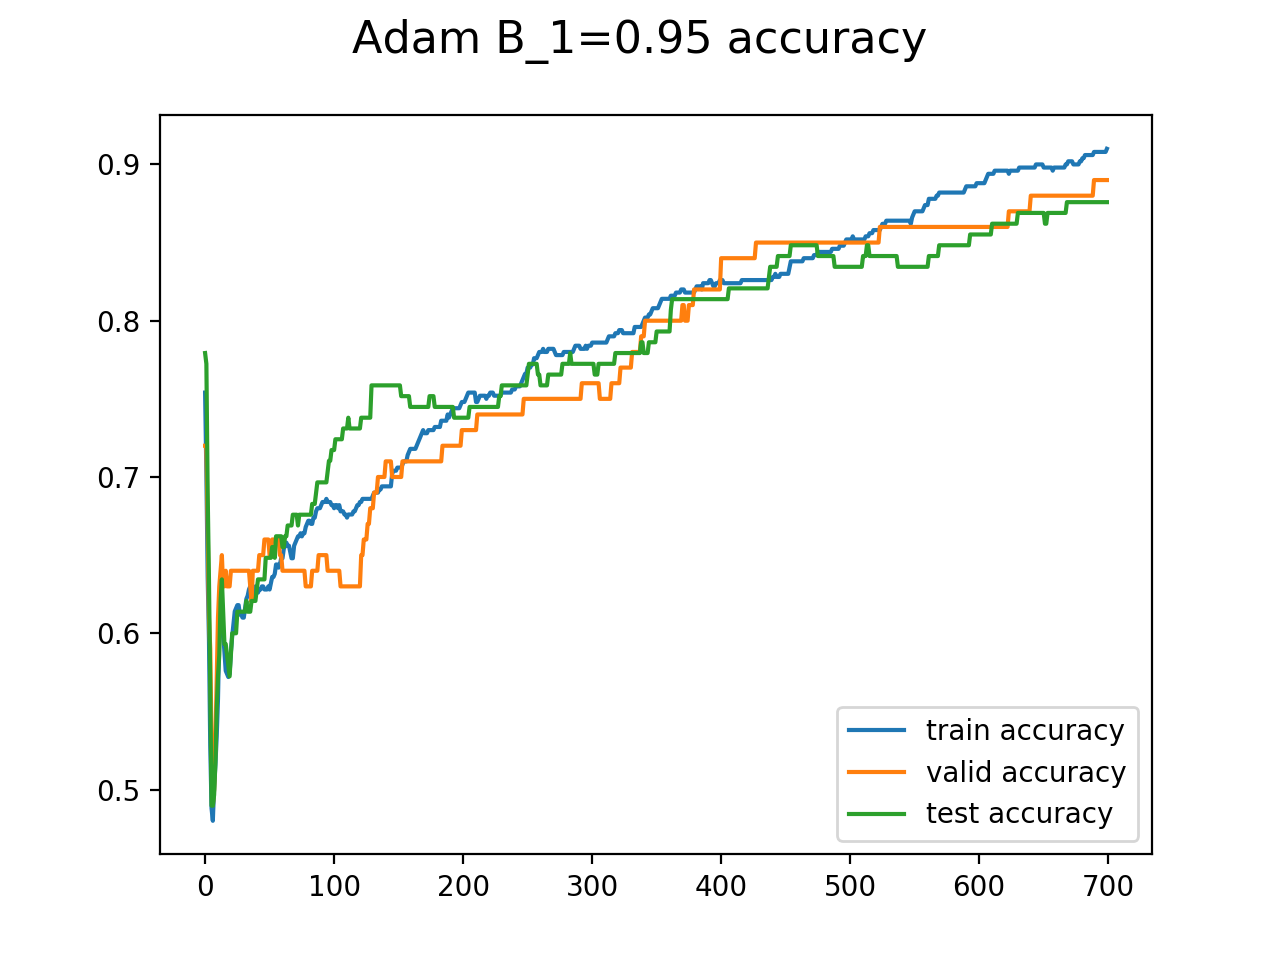
\includegraphics[width=.33\linewidth]{hyper_b11.png}\hfill
  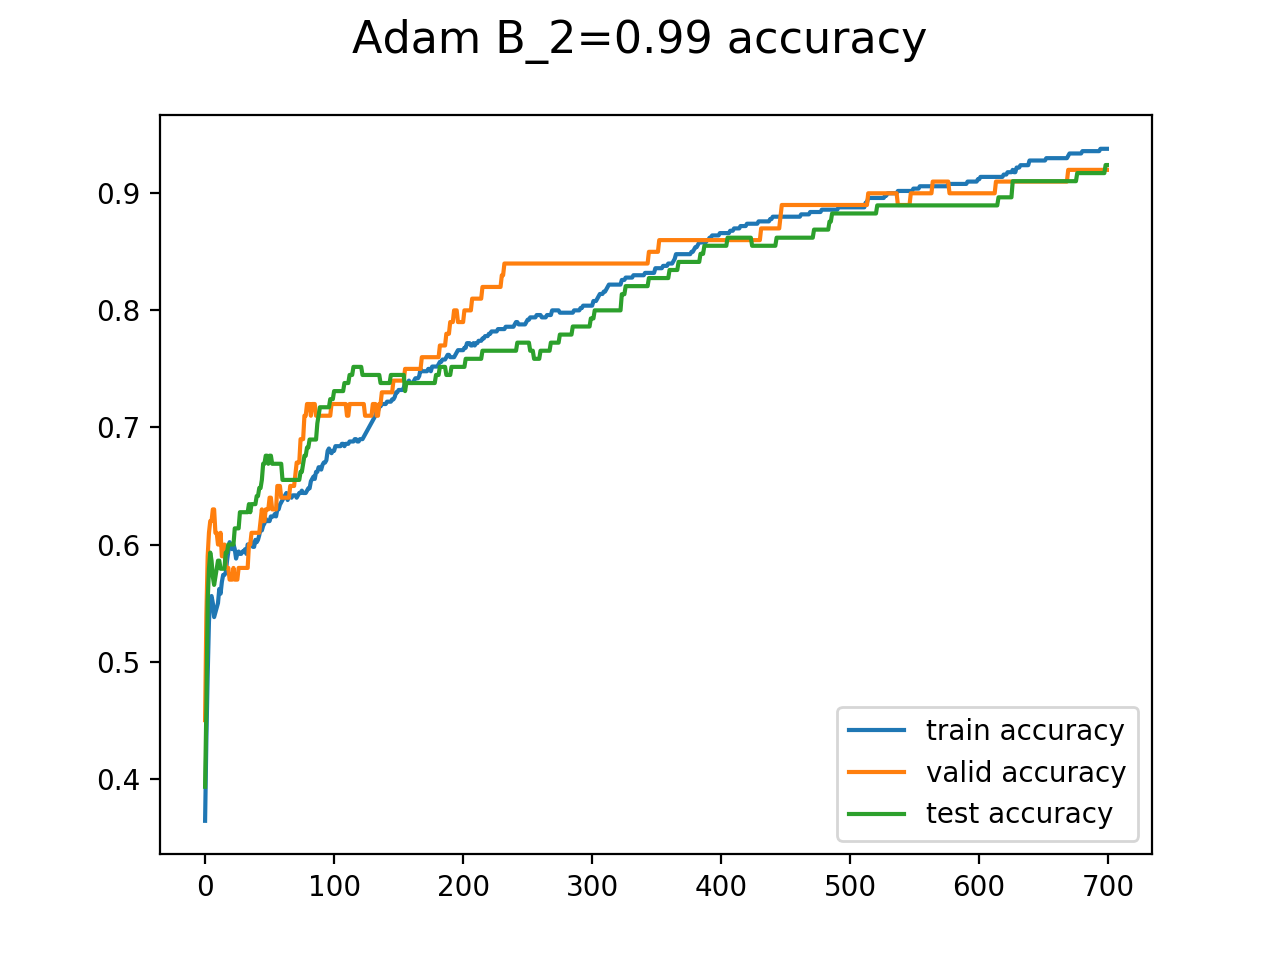
\includegraphics[width=.33\linewidth]{hyper_b21.png}\hfill
  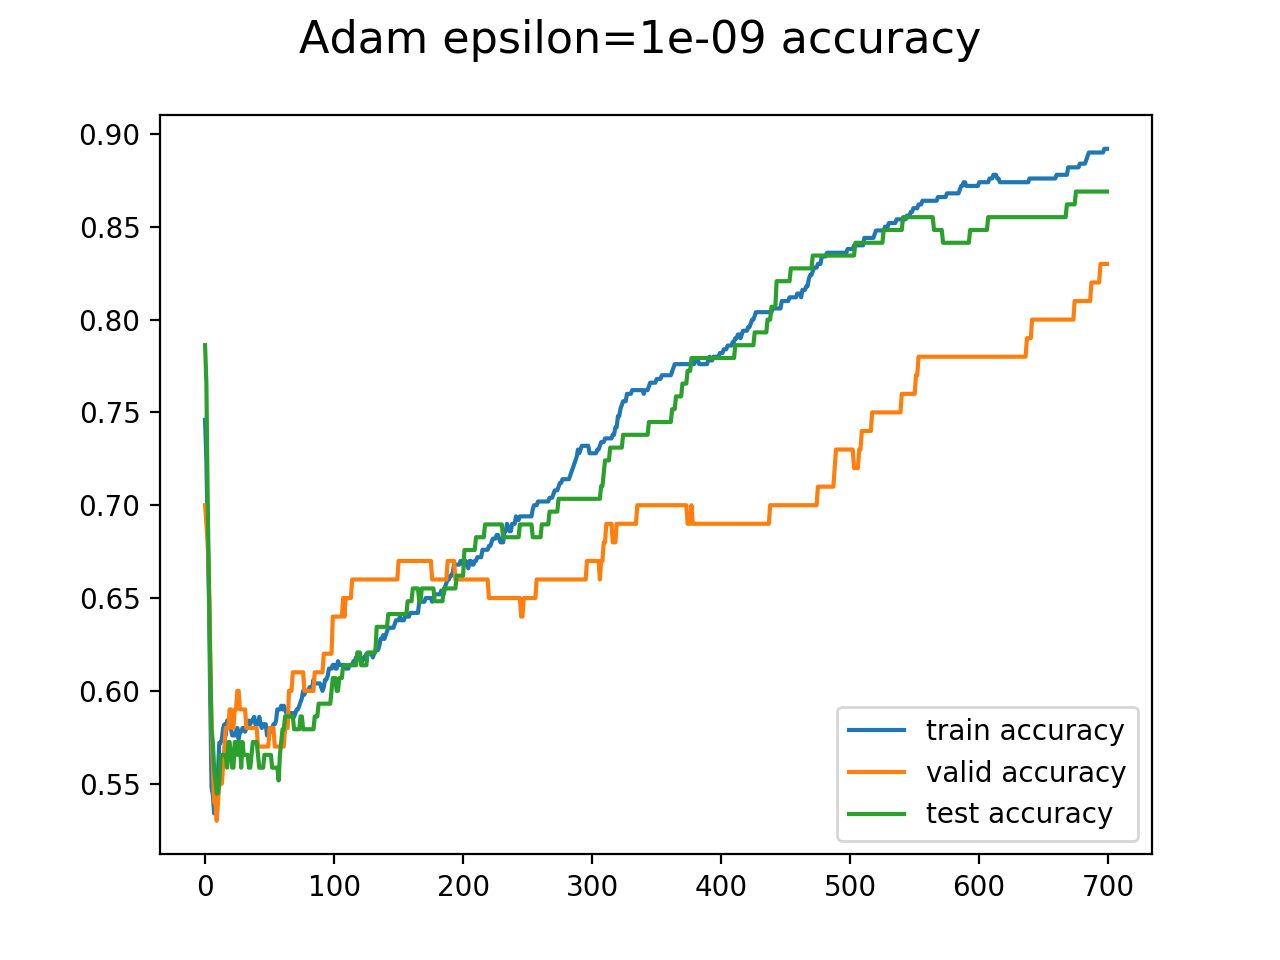
\includegraphics[width=.33\linewidth]{hyper_b31.png}\hfill
  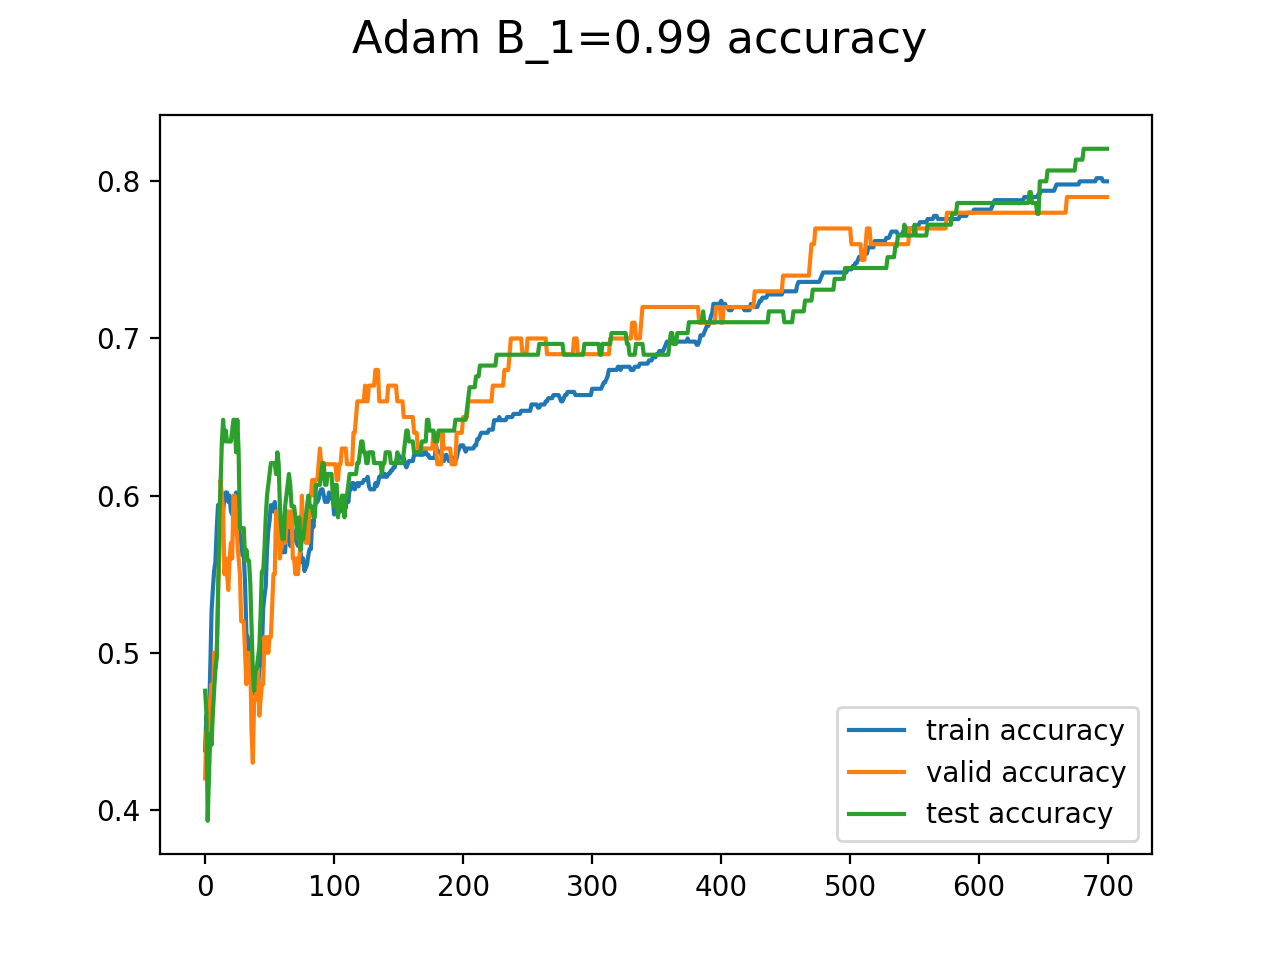
\includegraphics[width=.33\linewidth]{hyper_b12.png}\hfill
  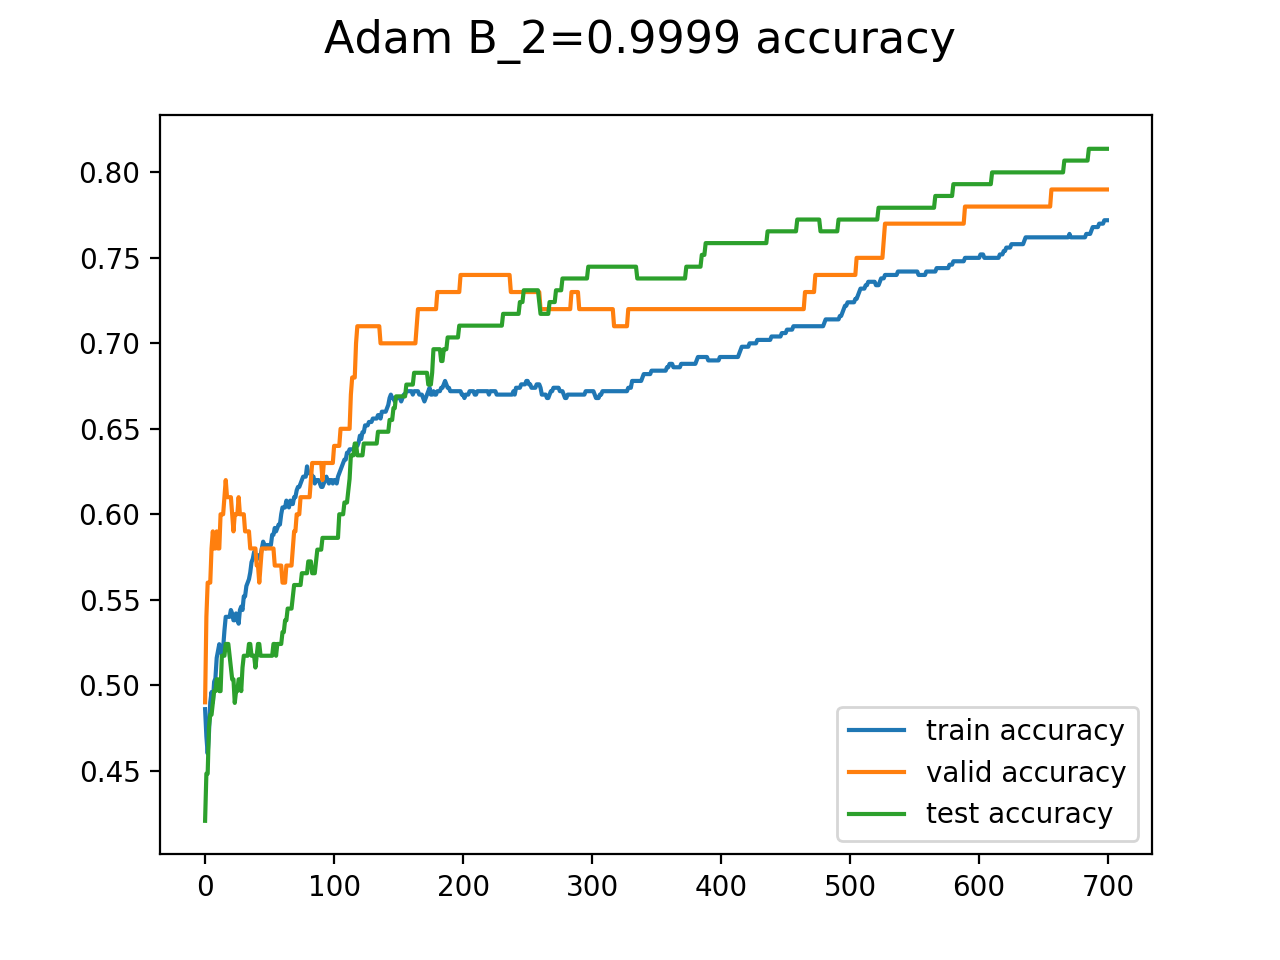
\includegraphics[width=.33\linewidth]{hyper_b22.png}\hfill
  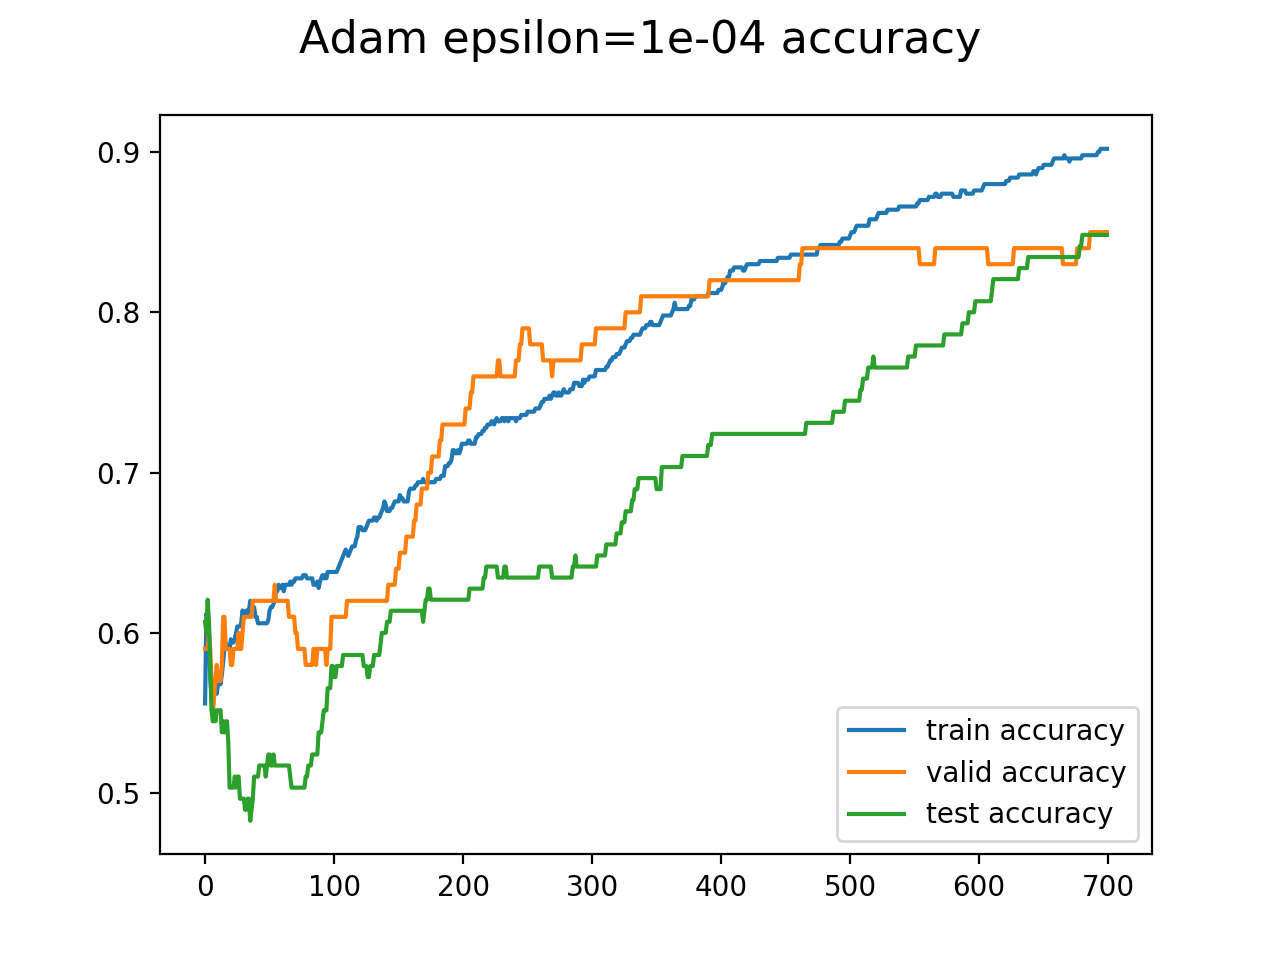
\includegraphics[width=.33\linewidth]{hyper_b32.png}\hfill
  \caption{Adam hyper parameter impact on Accuracy }
  \end{subfig}
\end{figure}


a) The Adam hyperparameter $\beta_1$ and $\beta_2$ are both use for speeding up the gradient decent. They are able to make the model converges faster than the standard gradient descent algorithm. $\beta_1$ is the exponential decay rate for the first moment estimates, which was adding momentum into consideration while doing gradient descent. By choosing a propriety value for $\beta_1$, each step size and direction were able to be adjusted, which led to faster convergent. first column on figure 9 had shown the accuracy curves plots with $\beta_1$ equals to 0.95 and 0.99. The 0.95 plot showed less oscillations at the beginning of the curves and reached a higher accuracy after 700 epochs. Since $\beta_1$ calculated current weight values by take historical values in to consideration. Higher the $\beta_1$ means more historical values had been took in for calculating the current weight values, therefore, when the $\beta_1$ equals 0.99, the model relaid heavily on the historical values (adding too much momentum), which gave less accuracy and more oscillations.\\

b) $\beta_2$ is the exponential decay rate for the second-moment estimates, it is similar as using Root Mean Square Propagation method when doing optimization. It works similar to the gradient descent algorithm for momentum ($\beta_1$), which could restrict the oscillation in the narrow direction and larger the steps in the wider direction. As shown in the figure 8 below, Vt is smaller when in the wider direction, and larger when in the narrow direction. Column 2 of Figure 9 had shown the accuracy curves for $\beta_2$ equals to 0.99 and 0.9999. As we can see, the accuracy was higher after 700 epochs with $\beta_2$ equals to 0.99 and lower when $\beta_2$ equals to 0.9999, and moreover, $\beta_2$ with value equals to 0.9999 was more inconsistent with train, valid, and test data accuracy curves. Is could also be explained by taken too much historical values while calculating new Vt, this had led to wrong direction taken for choosing the next weight.\\ 

c) $\epsilon$ value is a very small number to prevent a division by zero in the implementation. As shown in figure 8 above, the $\epsilon$ value was added to Vt in case Vt is equaling to zero. Column 3 of Figure 9 had shown the accuracy curves with $\epsilon$ equals to 1e-09 and 1e-04, as we could see, the over all accuracy for all three data sets are almost the same regardless of both $\epsilon$ values, however, curves for $\epsilon$ = 1e-09 has a big oscillation at the beginning of the curve, whereas the curves for $\epsilon$ = 1e-04 tend to be more smooth at the beginning. This met be caused by the zero initialize moment vectors, when $\epsilon$ = 1e-09 (very small number), there was less affect of $\epsilon$ towards weight parameters, therefore, there was oscillations at the beginning of the curves due to it had taken zero initialization into consideration. And when $\epsilon$ = 1e-04 (lager number), it is large enough to affect the update weights parameters.\\

Notice, the accuracy plots may various due to data were randomly shuffled every time when training. \\


\subsection{Cross Entropy Loss Investigation}

\begin{figure}[H]
\centering
 \begin{subfig}
  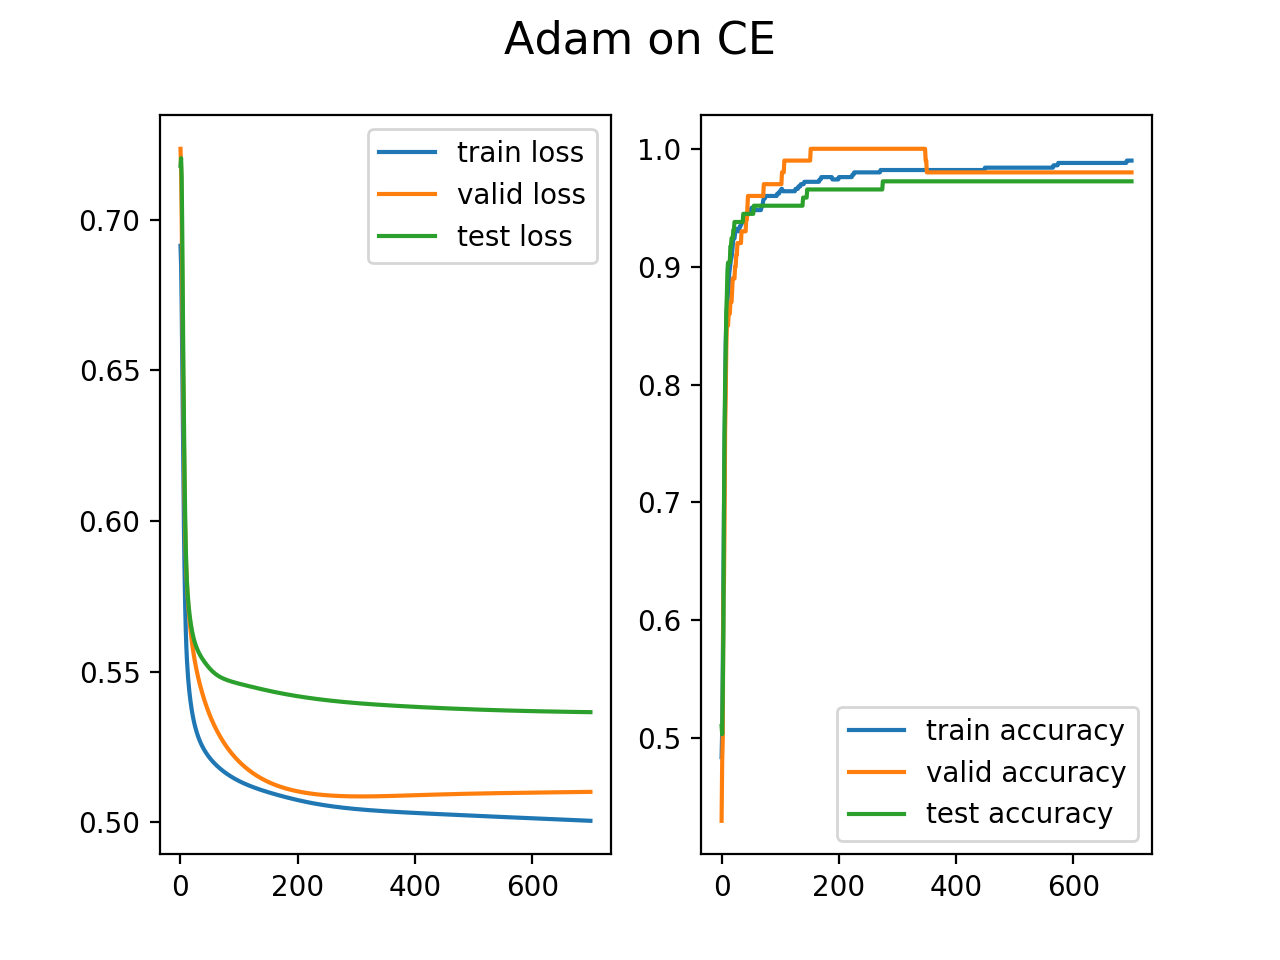
\includegraphics[width=.45\linewidth]{adam_CE.png}\hfill
  \caption{Minimizing binary cross entropy loss using Adam}
  \end{subfig}
\end{figure}



\begin{figure}[H]
\centering
 \begin{subfig}
  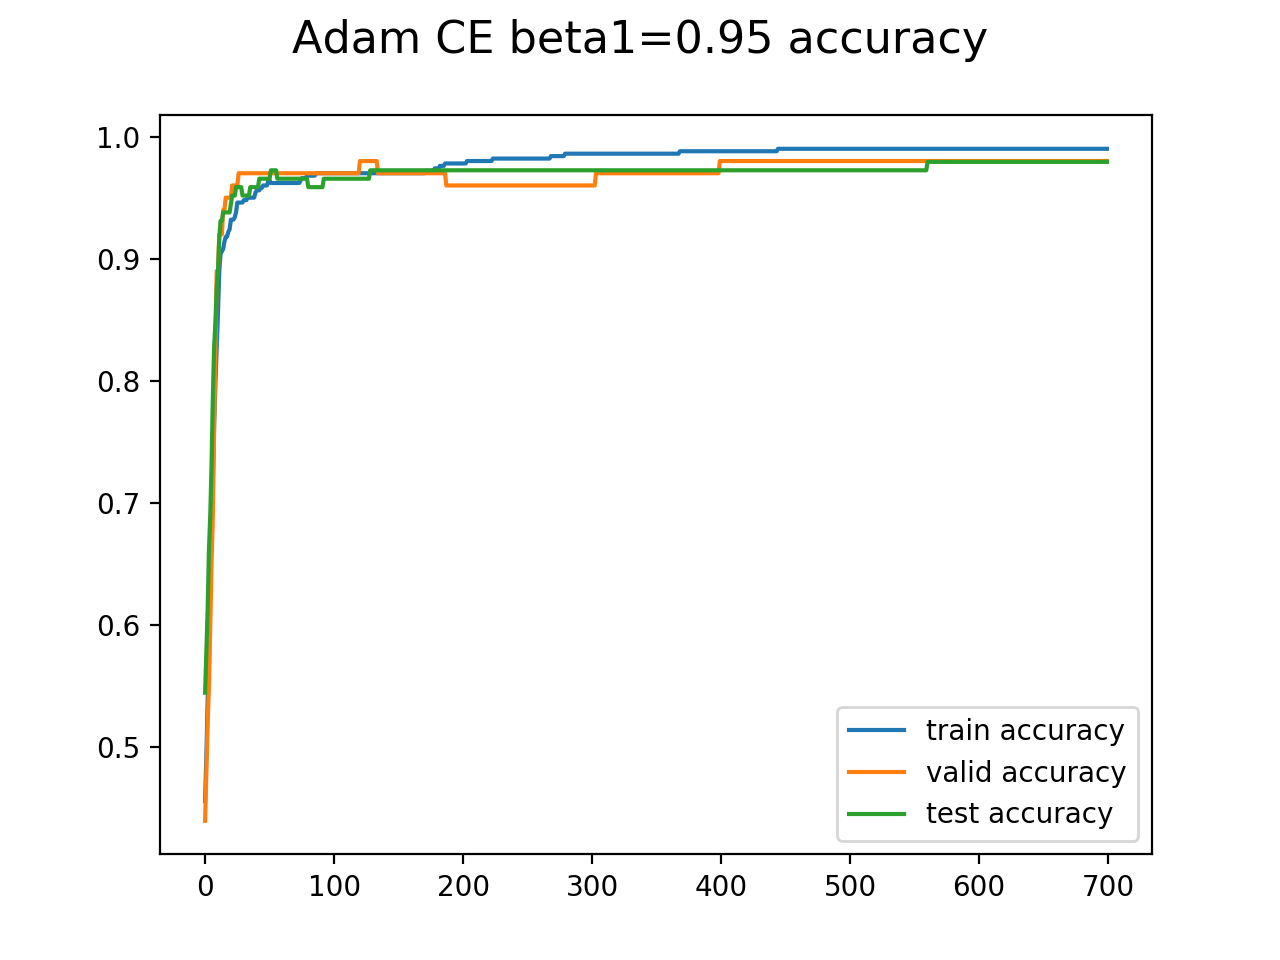
\includegraphics[width=.33\linewidth]{hyper_b11_CE.png}\hfill
  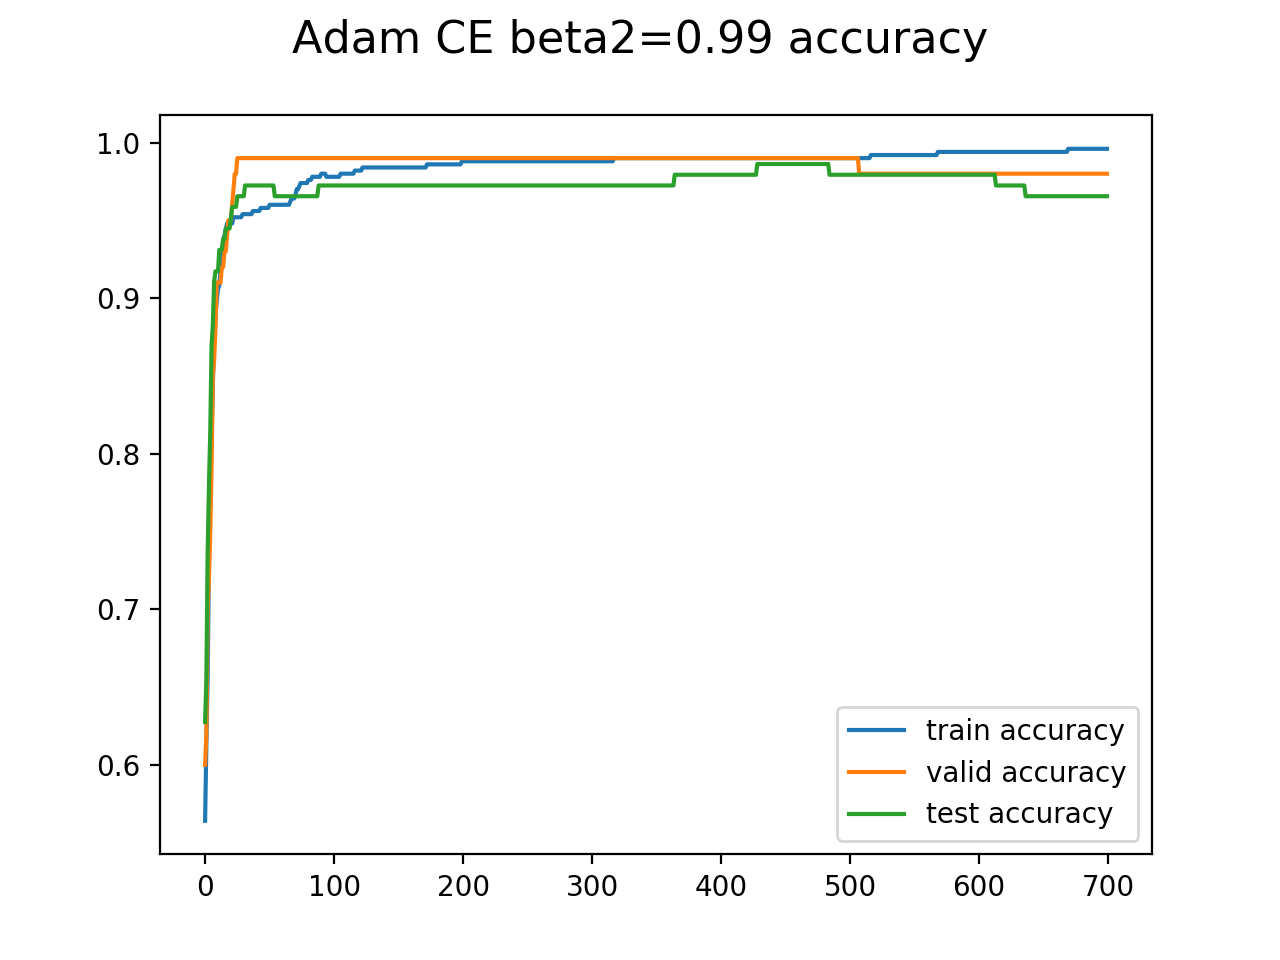
\includegraphics[width=.33\linewidth]{hyper_b21_CE.png}\hfill
  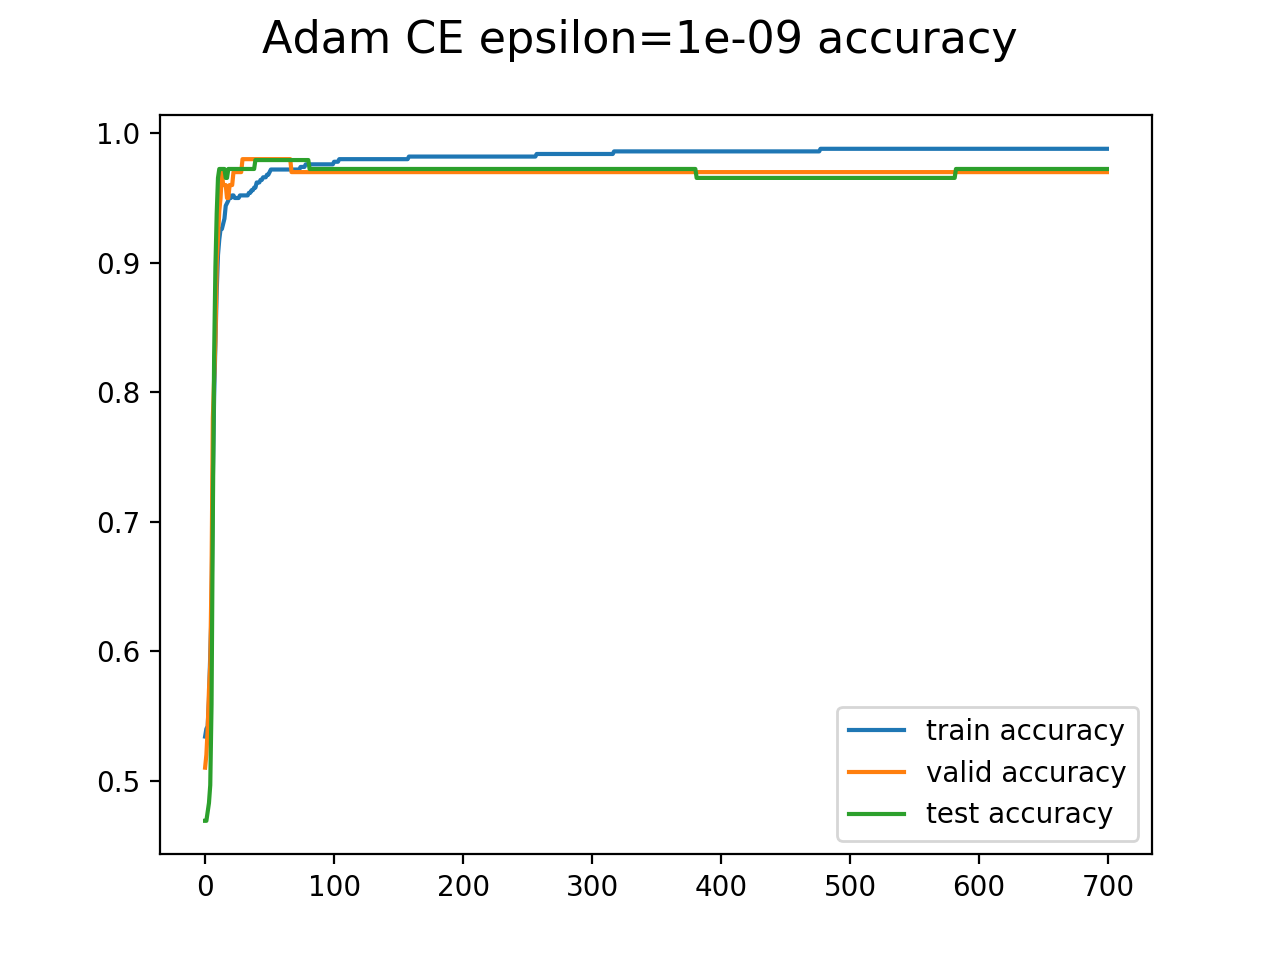
\includegraphics[width=.33\linewidth]{hyper_b31_CE.png}\hfill
  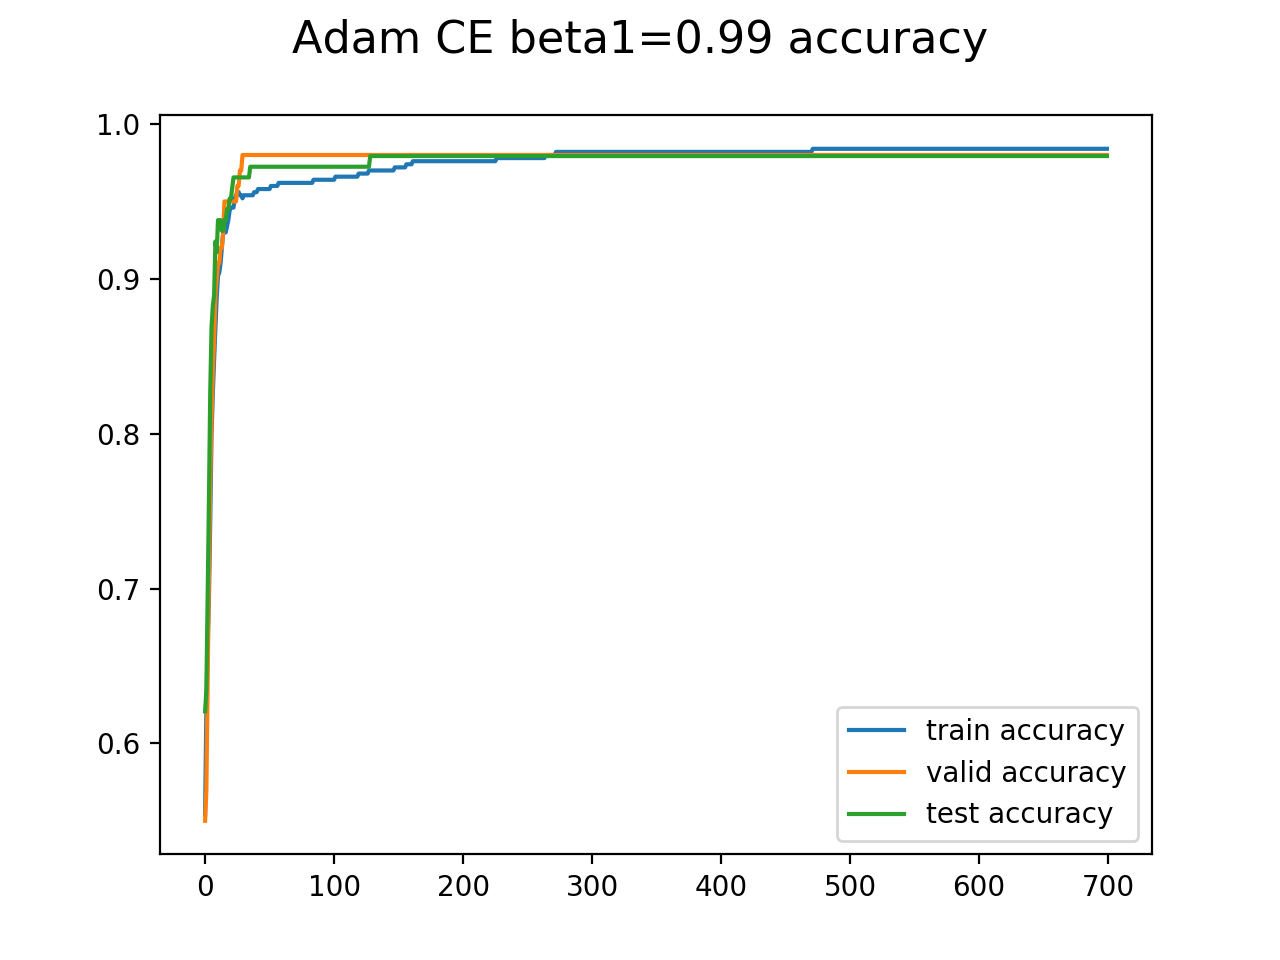
\includegraphics[width=.33\linewidth]{hyper_b12_CE.png}\hfill
  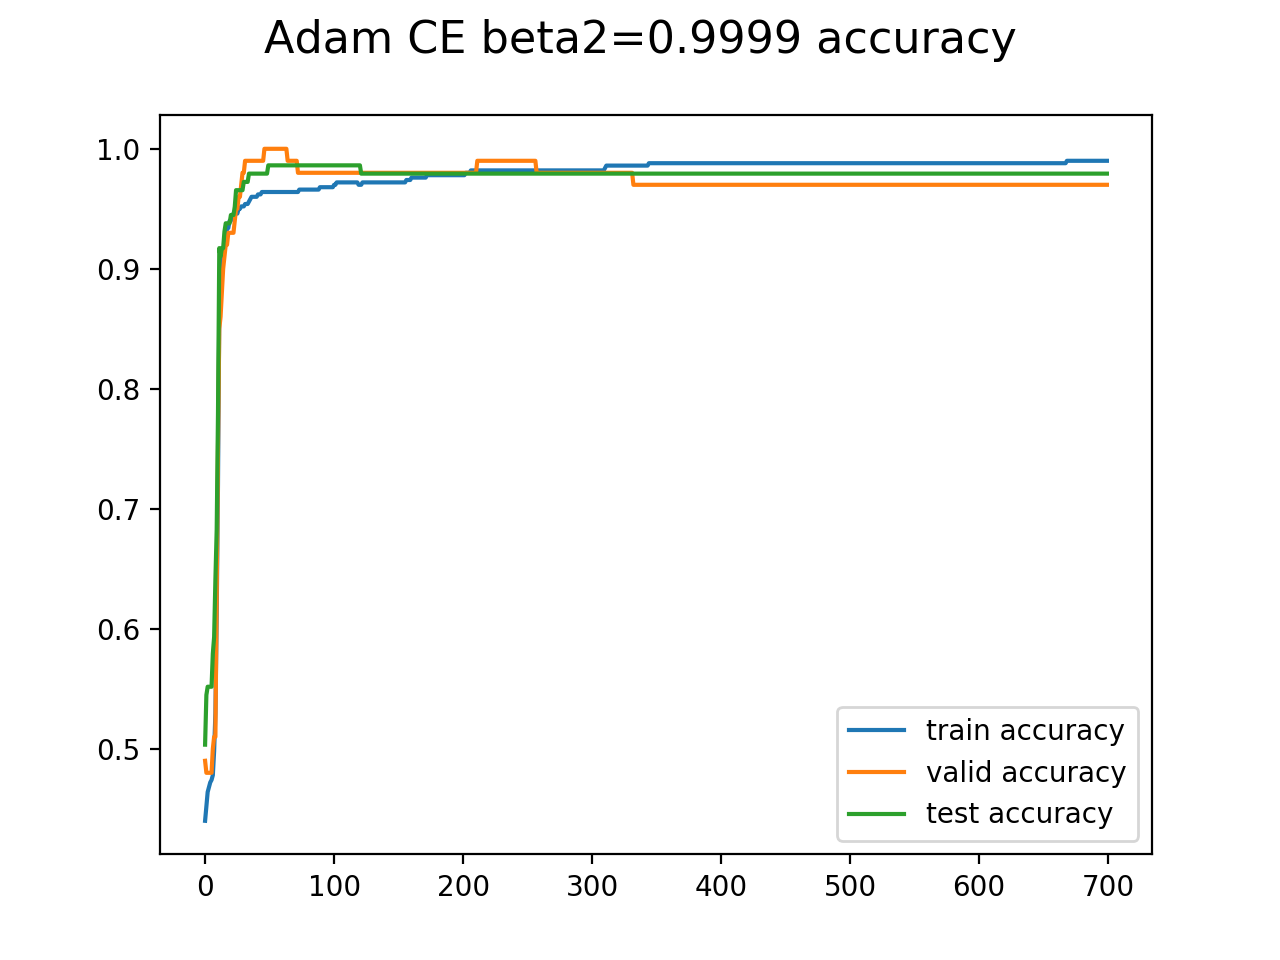
\includegraphics[width=.33\linewidth]{hyper_b22_CE.png}\hfill
  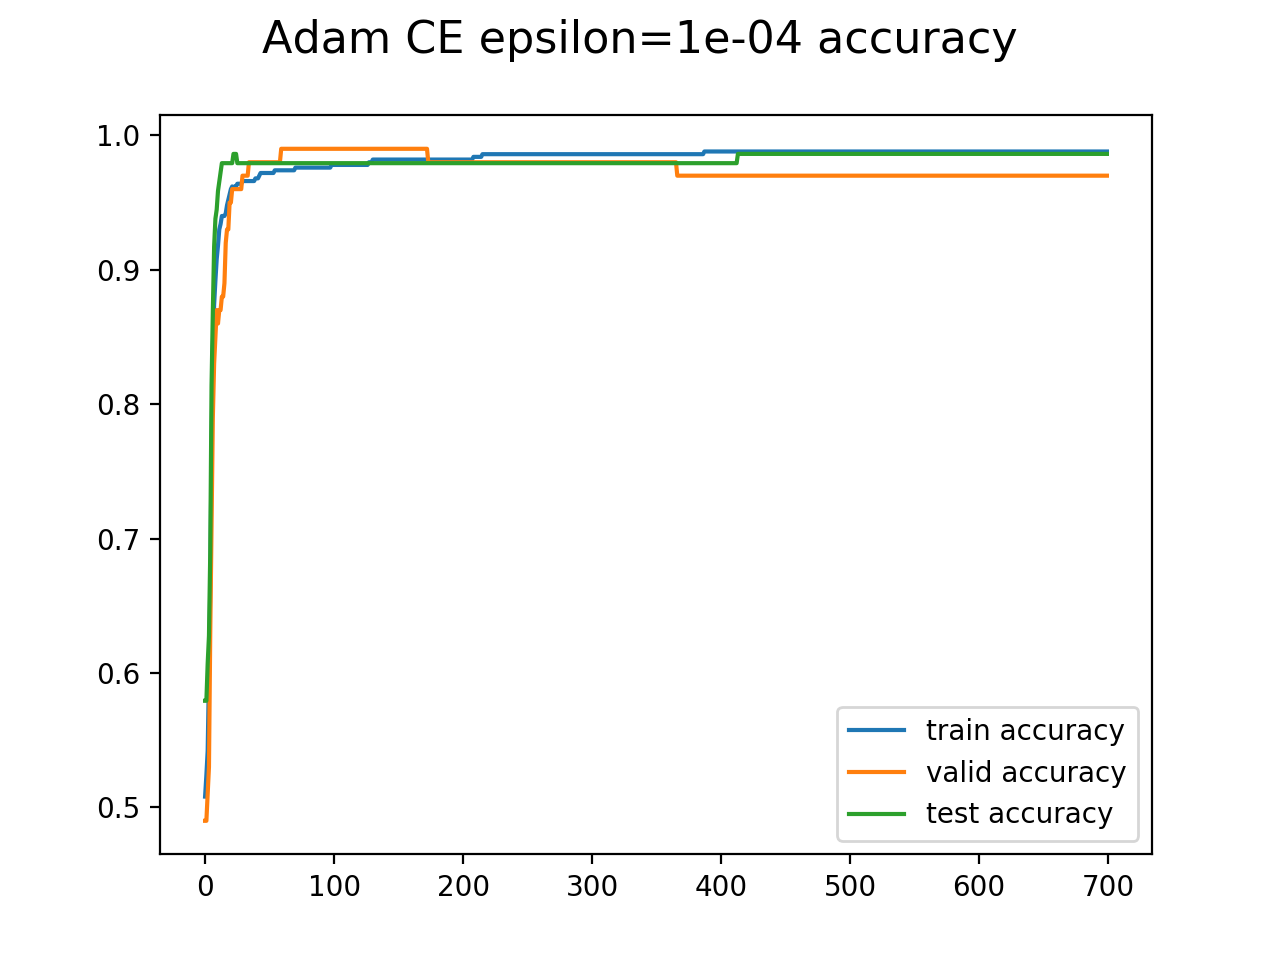
\includegraphics[width=.33\linewidth]{hyper_b32_CE.png}\hfill
  \caption{Adam hyper parameter impact on Accuracy on Cross Entropy}
  \end{subfig}
\end{figure}




\qquad Figure 10 had shown the loss curves and accuracy curves for model using Adam cross entropy, compares to the model using MSE approach (Figure 6), the losses with CE model had starting at a much lower number (0.75 vs 25) and had faster decay. On the other side, for accuracy curves, instead of approximately 0.75 accuracy for MSE model, CE had reached close to one in fewer epochs. CE model also had higher consistency for the accuracy curves in all train, valid, and test data, which means it trained the model better than MSE. For changed $\beta_1$, $\beta_2$ or $\epsilon$ values on figure 10 for CE compared to figure 9 for MSE, CE approach had shown higher accuracy in every case compared to using MSE, and the affect of change in hyper-parameter for CE were very small. A possible reason for that was CE approach can reach a optimum training model with in 700 epochs much faster, therefore, less need for to speed up (optimization).


\begin{table}[H]
\centering
\begin{tabular}{|c|c|c|c|c|c|c|}
\hline
        &  \beta_1 = 0.95      &  \beta_1 = 0.99 &  \beta_2 = 0.99  & \beta_2 = 0.9999 & \epsilon = 1e-9 & \epsilon = 1e-4  \\ \hline
Train data accuracy & 99\% & 98.4\%  & 99.6\% & 99\%  &  98.8\% & 98.8\% \\ \hline
Valid data accuracy    & 98\% & 98\%  & 98\% & 97\%  &  97\% & 97\%   \\ \hline
Test data accuracy & 98\% & 98\%  & 96.6\% & 98\%  &  97.2\% & 98.6\% \\
\hline
\end{tabular}
\caption{Different Hyper-parameters final accuracy.}
\end{table}


\subsection{Comparison against Batch GD} 

\qquad Due to smaller batch sizes and the Adam optimizer effect, the overall performance for training model using SGD algorithm with Adam is much better than using batch gradient decent algorithm that we had implemented in part 1 and 2. \textbf{In addition, for the loss plots:}\\

Batch GD algorithm: 
\begin{quote}
    - Loss for MSE (figure 2) was starting around 60 and reached almost zero after 5000 epochs.\\
   - Loss for CE (figure 4) was starting around 40 and reached almost zero after 5000 epochs.
\end{quote}
    


SGD algorithm with Adam:  
\begin{quote}
    - Loss for MSE (figure 6) was starting around 25 and reached almost zero after 700 epochs.\\
   - Loss for CE (figure 10) was starting around 0.75 and reached almost zero after 700 epochs.
\end{quote}


We could see SGD with Adam has much lower loss in each cases compared to use batch GD algorithm.\\
\\
\textbf{For the accuracy plots:}\\

Batch GD algorithm: 
\begin{quote}
- Accuracy for MSE (figure 2) was very inconsistent with three data sets and reached around 0.65 accurate after 5000 epochs. \\
- Accuracy for CE (figure 4) was consistent with three data sets and reached around 1.0 accurate after 5000 epochs.
\end{quote}


SGD algorithm with Adam:
\begin{quote}
    - Accuracy for MSE (figure 6) was very inconsistent with three data sets and reached around 0.75 accurate after 700 epochs.\\
- Accuracy for CE (figure 10) was consistent with three data sets and reached around 1.0 accurate after 700 epochs.
\end{quote}

We could see SGD algorithm with Adam improved the final accuracy for MSE approach. For CE approach, there was not much difference between batch GD and SGD algorithms.\\

There are several possible explanations of why SGD with Adam gives a general better performance in perspectives of speed, loss, and accuracy. firstly, by using smaller sized batches, the calculation time will be much faster compared to use the whole data set to compute. Secondly, by using the Adam optimizer, it could lead to a faster convergence rate by using a more accurate step direction towards minimum value. Thirdly, Adam optimizer can also adds momentum when determining Weights, which helped the model to escape shallow local minimums. 
\\
\medskip
\vspace{15mm}

\bibliographystyle{ieeetr}
\bibliography{samples}



\end{document}
